\section{Hardware Implementation}\label{hwi}
\subsection{What we did}\label{wwd}
As described in the introduction, we focused on replicating the interference shown in \cite{Fu18} through electromagnetic coupling between an emitter and a thermocouple. The equipment used was as follows: RIGOL DG4162 Function Generator \cref{fig:FGen}, 30-turn copper inductor (\cref{fig:Inductor}), 6-in Type-K thermocouple \cref{fig:Thermocouple}, MAX31856 thermocouple breakout board \cref{fig:MAX31856}, and a Tektronix DPO 3034 oscilloscope on the thermocouple outputs \cref{fig:DPO3034}. No modifications were performed on the equipment. The basic setup for our experiments is shown in \cref{fig:Block}.

% % Here is how to insert a picture
% \begin{figure}
% \label{this-is-my-label}
% \includegraphics{fly}
% \caption{A sample black and white graphic.}
% \end{figure}
\begin{figure}
    \centering
    \includegraphics[width=\linewidth]{Function-Gen-Pic.jpg}
    \caption{RIGOL DG4162}
    \label{fig:FGen}
\end{figure}
\begin{figure}
    \centering
    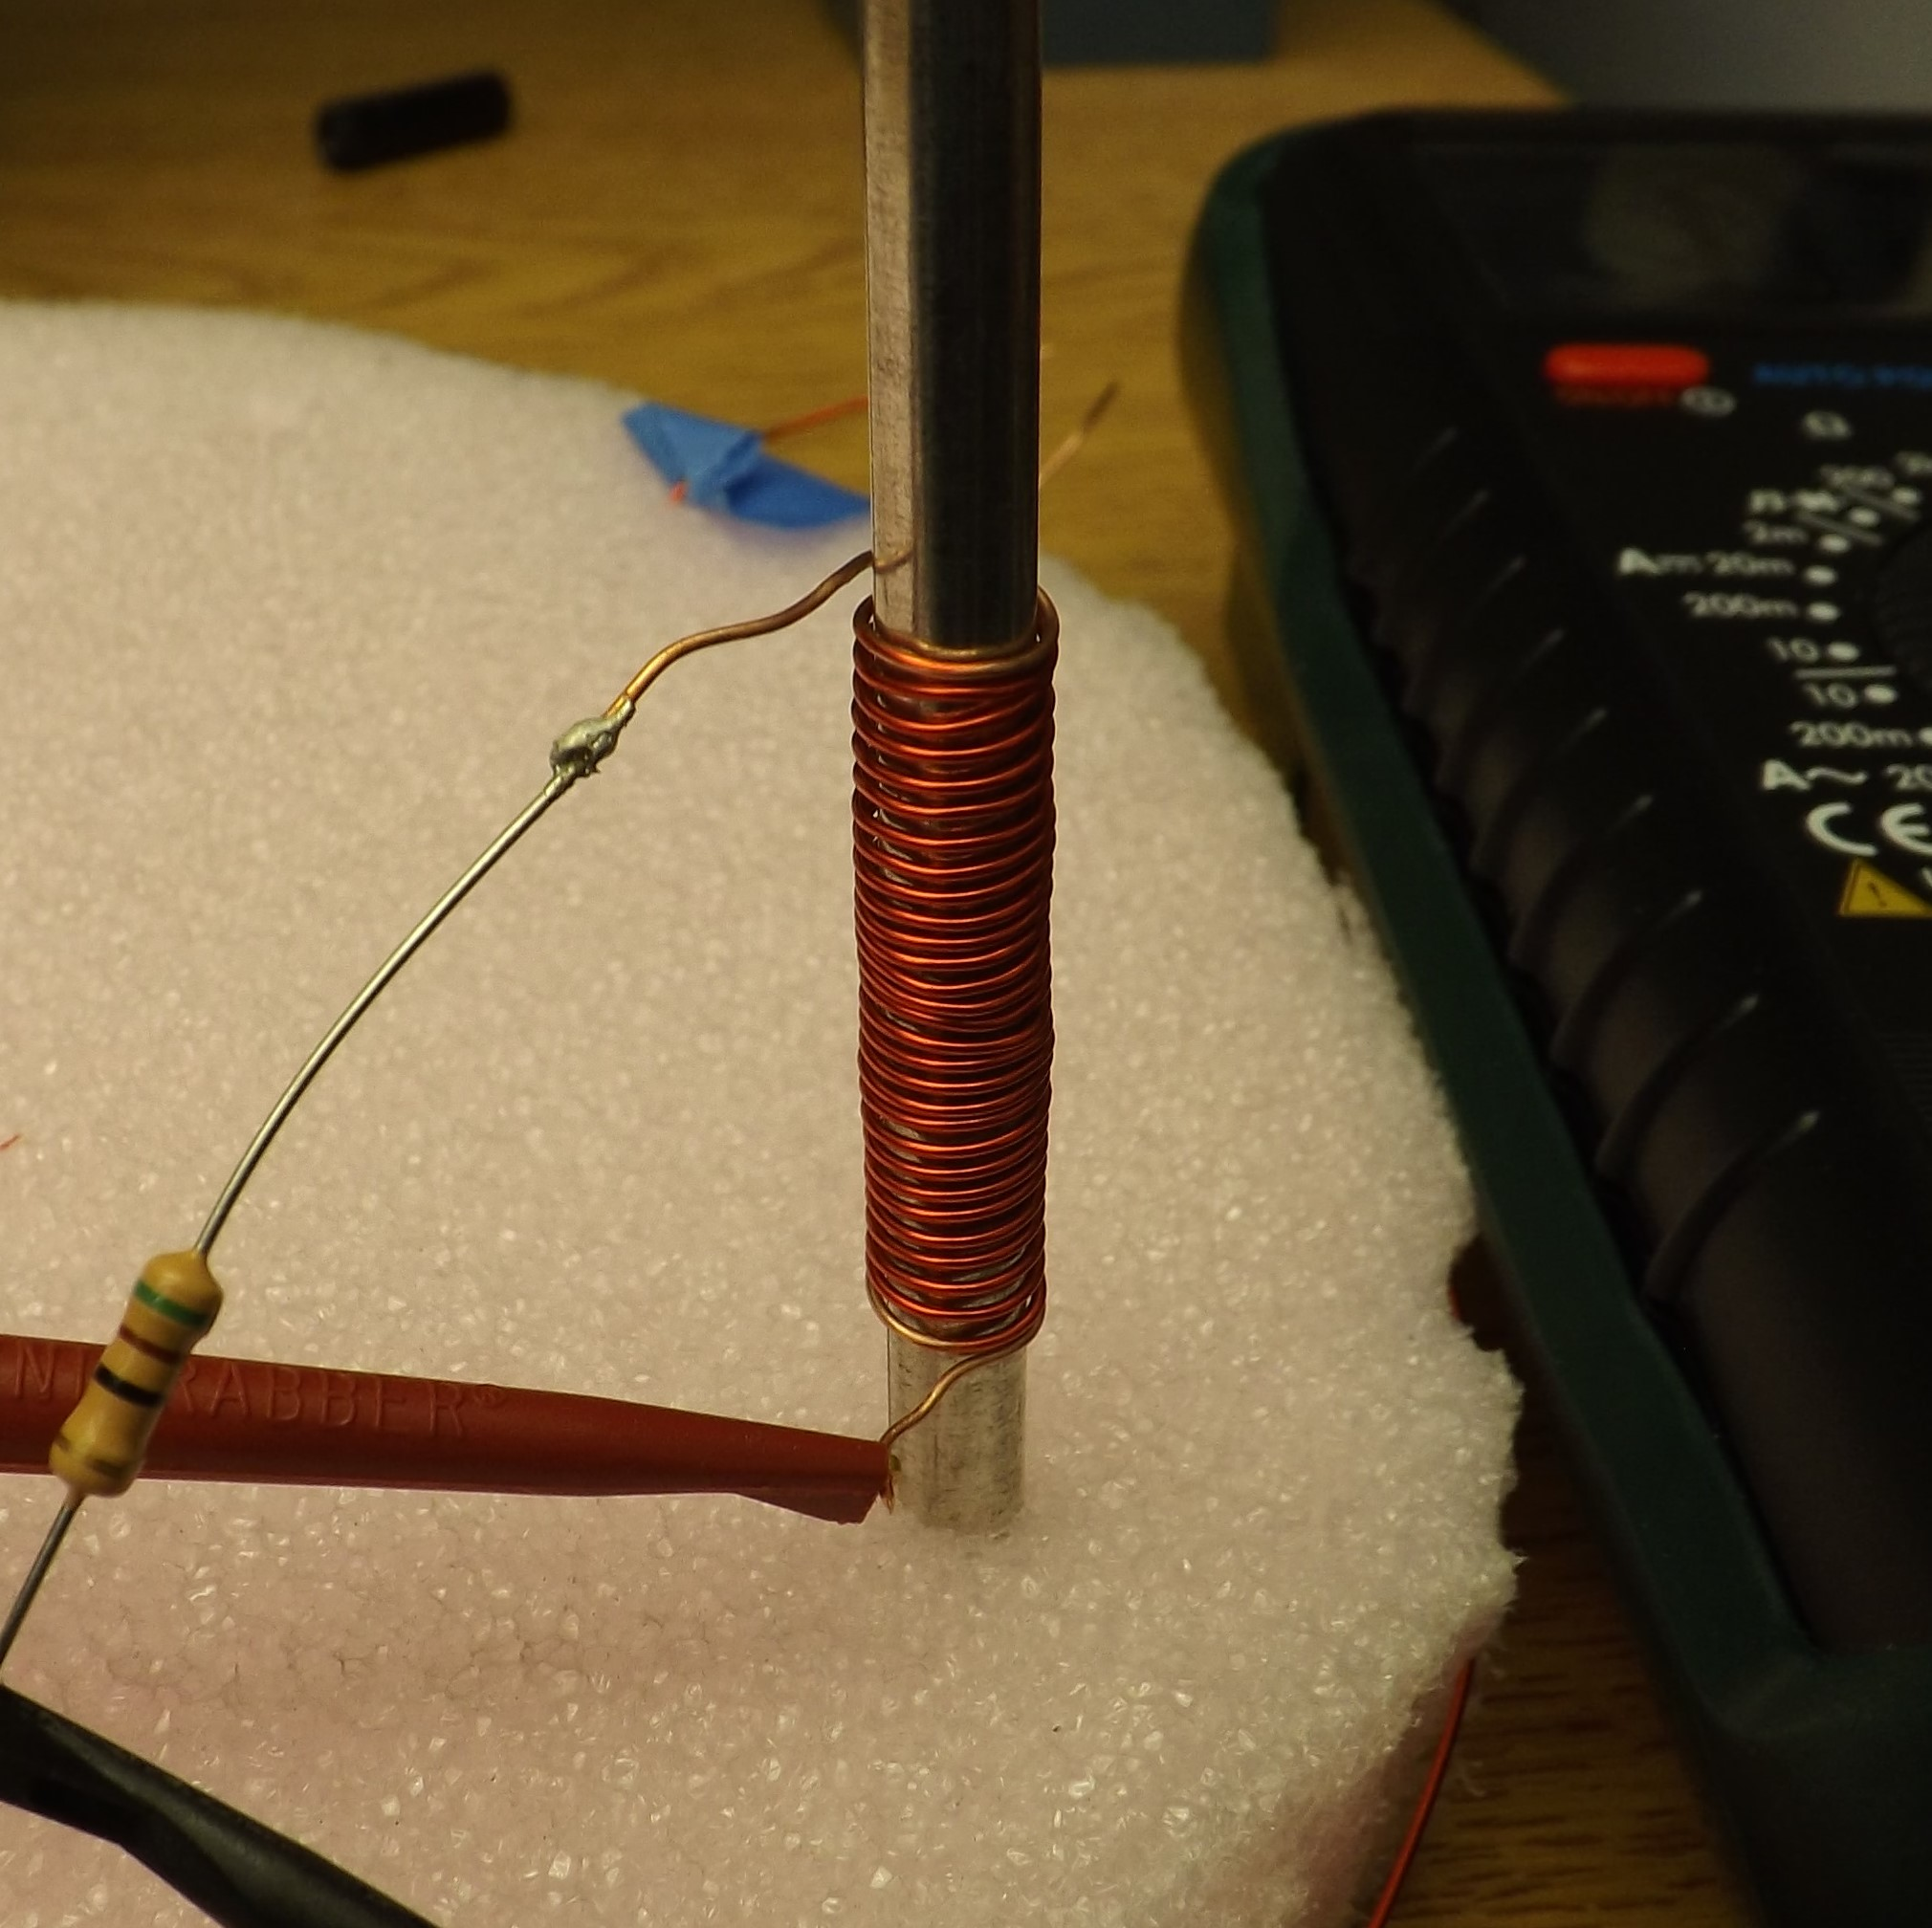
\includegraphics[width=\linewidth]{Inductor-Close-Up.jpg}
    \caption{30-Turn Copper Inductor}
    \label{fig:Inductor}
\end{figure}
\begin{figure}
    \centering
    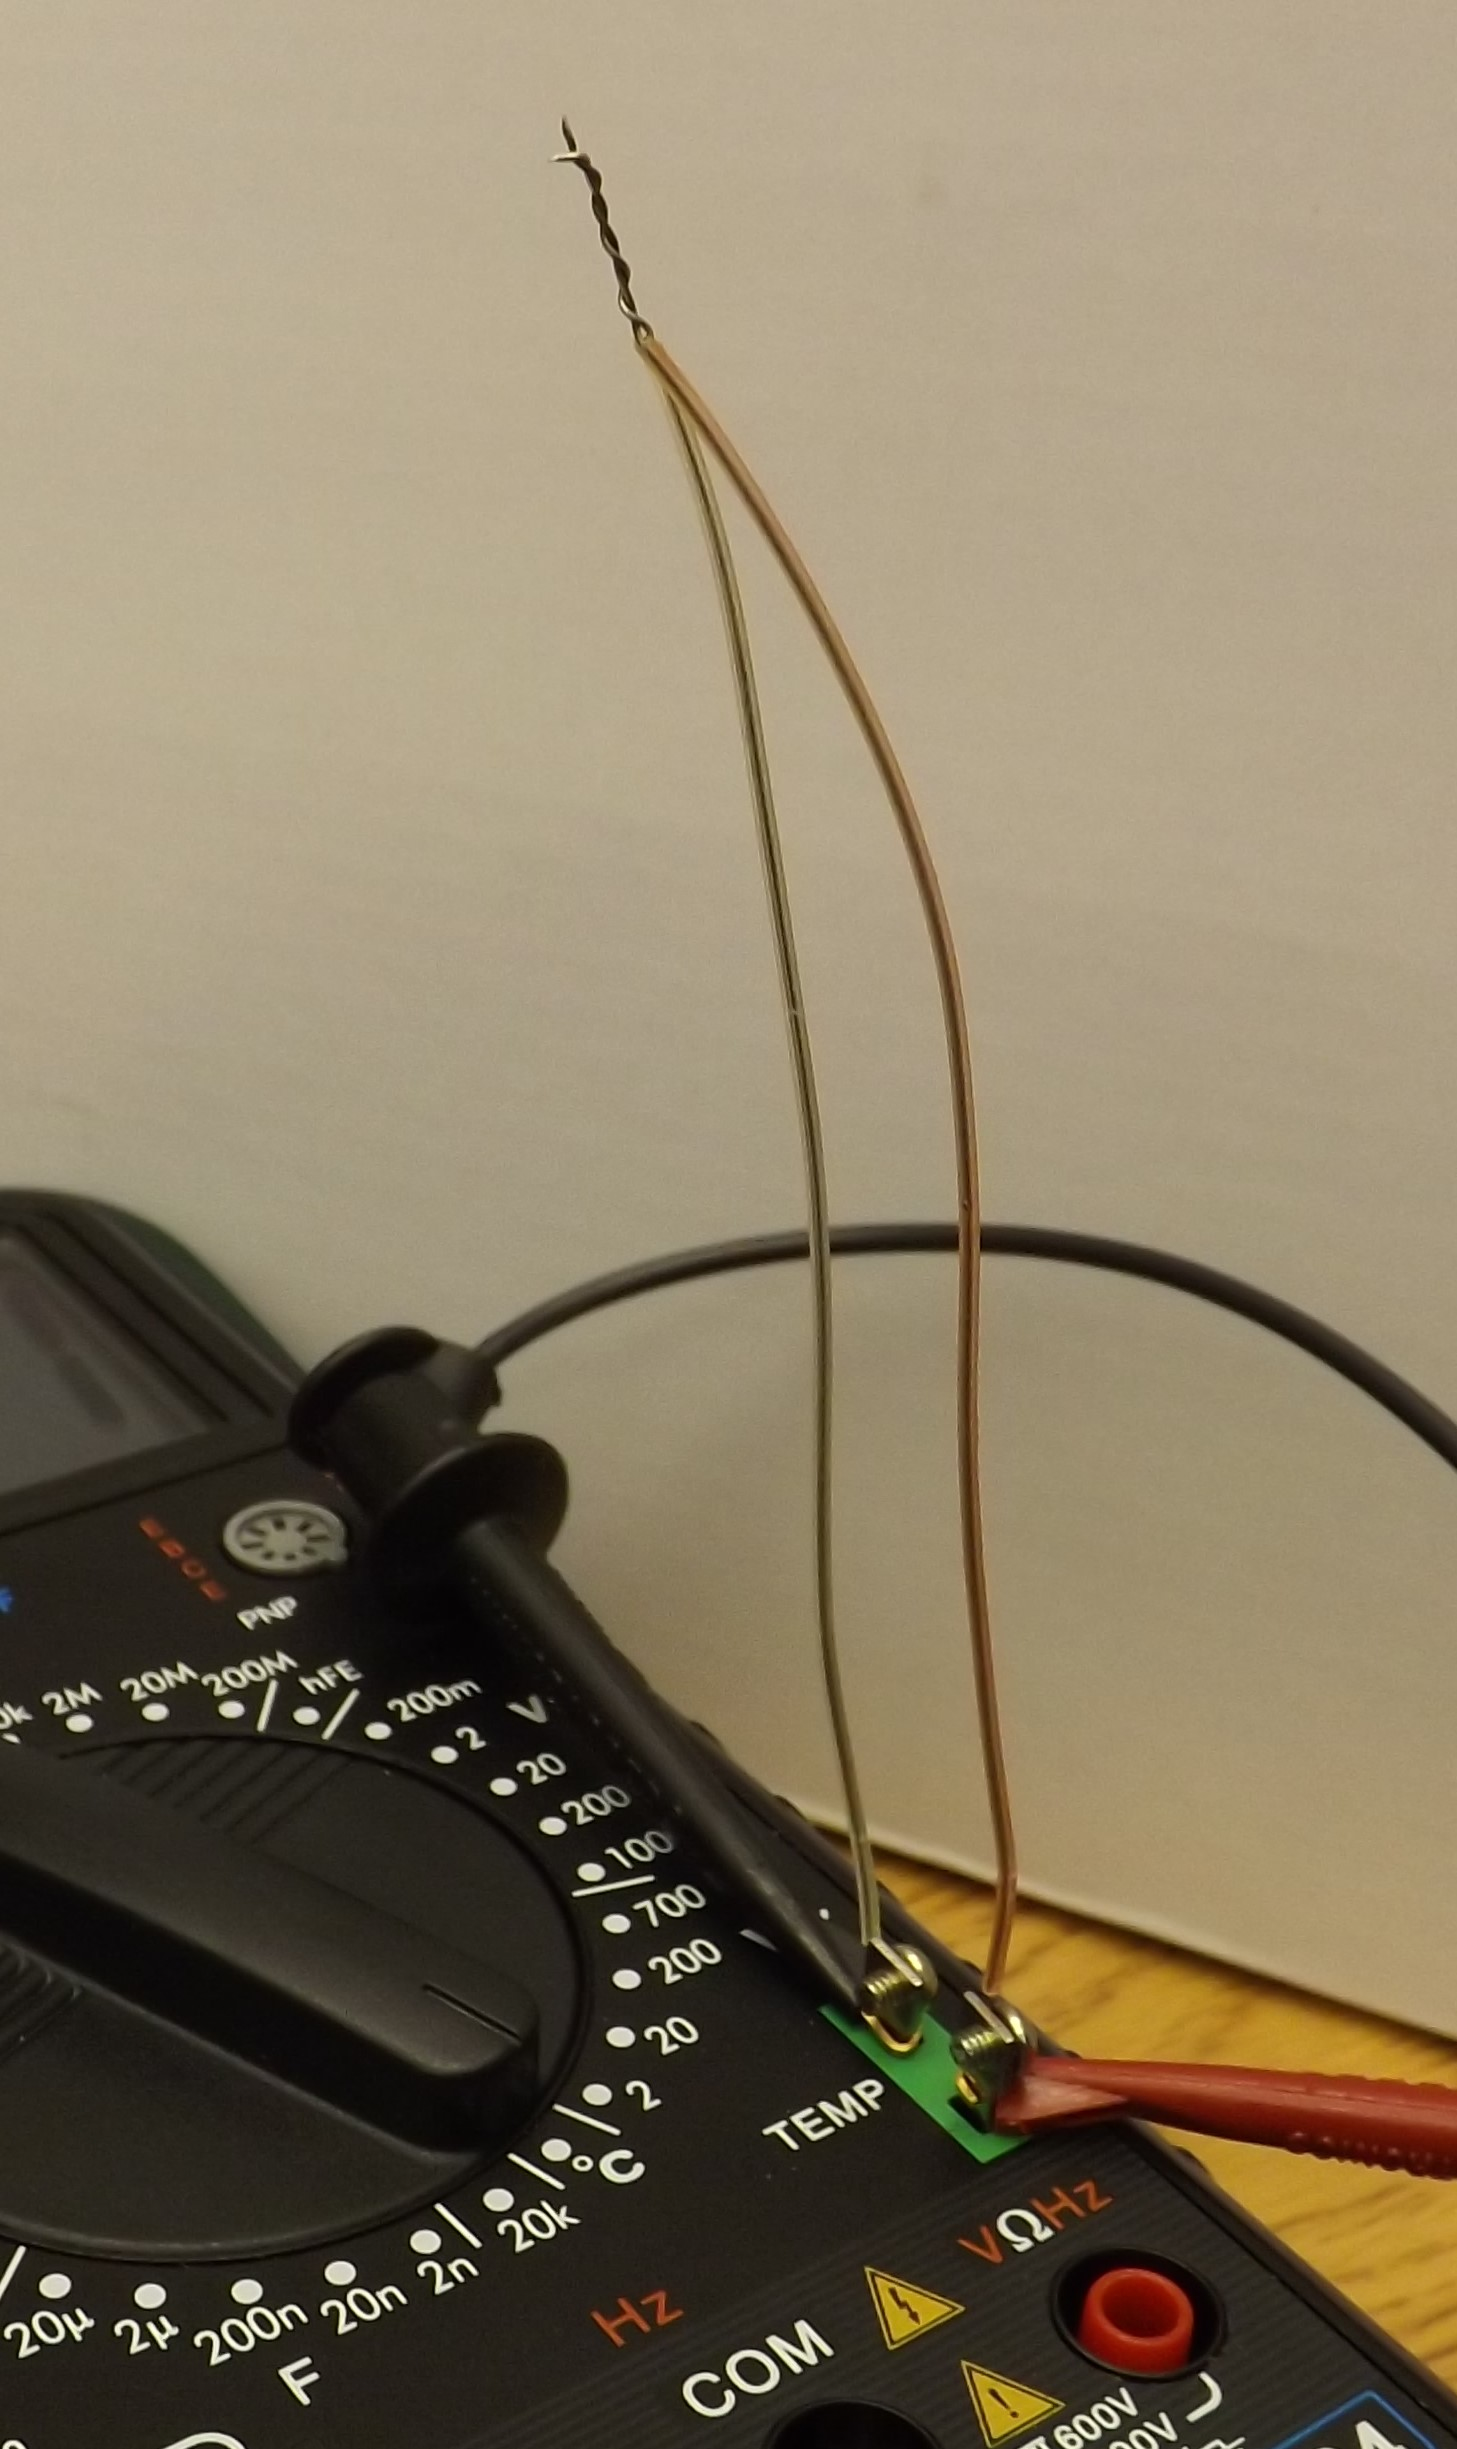
\includegraphics[width=.5\linewidth]{Thermocouple.jpg}
    \caption{Type-K Thermocouple}
    \label{fig:Thermocouple}
\end{figure}
\begin{figure}
    \centering
    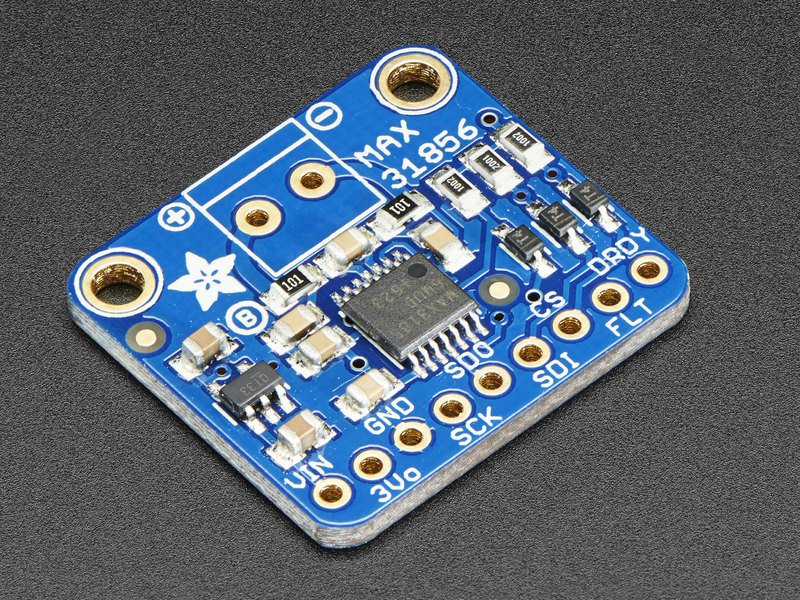
\includegraphics[width=0.75\linewidth]{MAX31856.jpg}
    \caption{MAX31856 Breakout Board}
    \label{fig:MAX31856}
\end{figure}
\begin{figure}
    \centering
    \includegraphics[width=\linewidth]{DPO3034.jpg}
    \caption{Tektronix DPO 3034}
    \label{fig:DPO3034}
\end{figure}
\begin{figure}
    \centering
    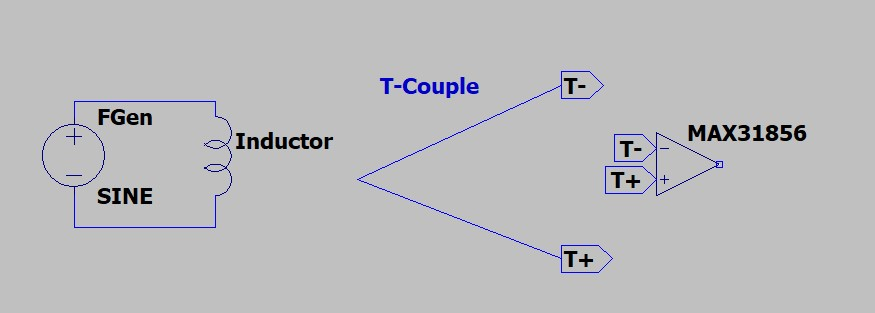
\includegraphics[width=\linewidth]{Block-Diagram.jpg}
    \caption{Experiment Setup Block Diagram}
    \label{fig:Block}
\end{figure}

Using the function generator, we performed a frequency sweep from 10Hz to 70 MHz at 10$V_{pp}$ to see which frequencies were the most apparent on the output. From the sweep, the thermocouple showed the most response at 47Mhz \cref{fig:47mhz,fig:InductorThermocouple,fig:Osci47,fig:Osci47-2}. As is shown in the figures, the thermocouple is showing a 47MHz at 202$mV_{pp}$ signal without being directly connected to the function generator. However, this signal did not translate to a change in the temperature output of the MAX31856. Instead of showing the temperature corresponding to the induced $V_{pp}$ signal as was expected, the thermocouple continued to operate normally, registering real temperate changes that were performed.

\begin{figure}
    \centering
    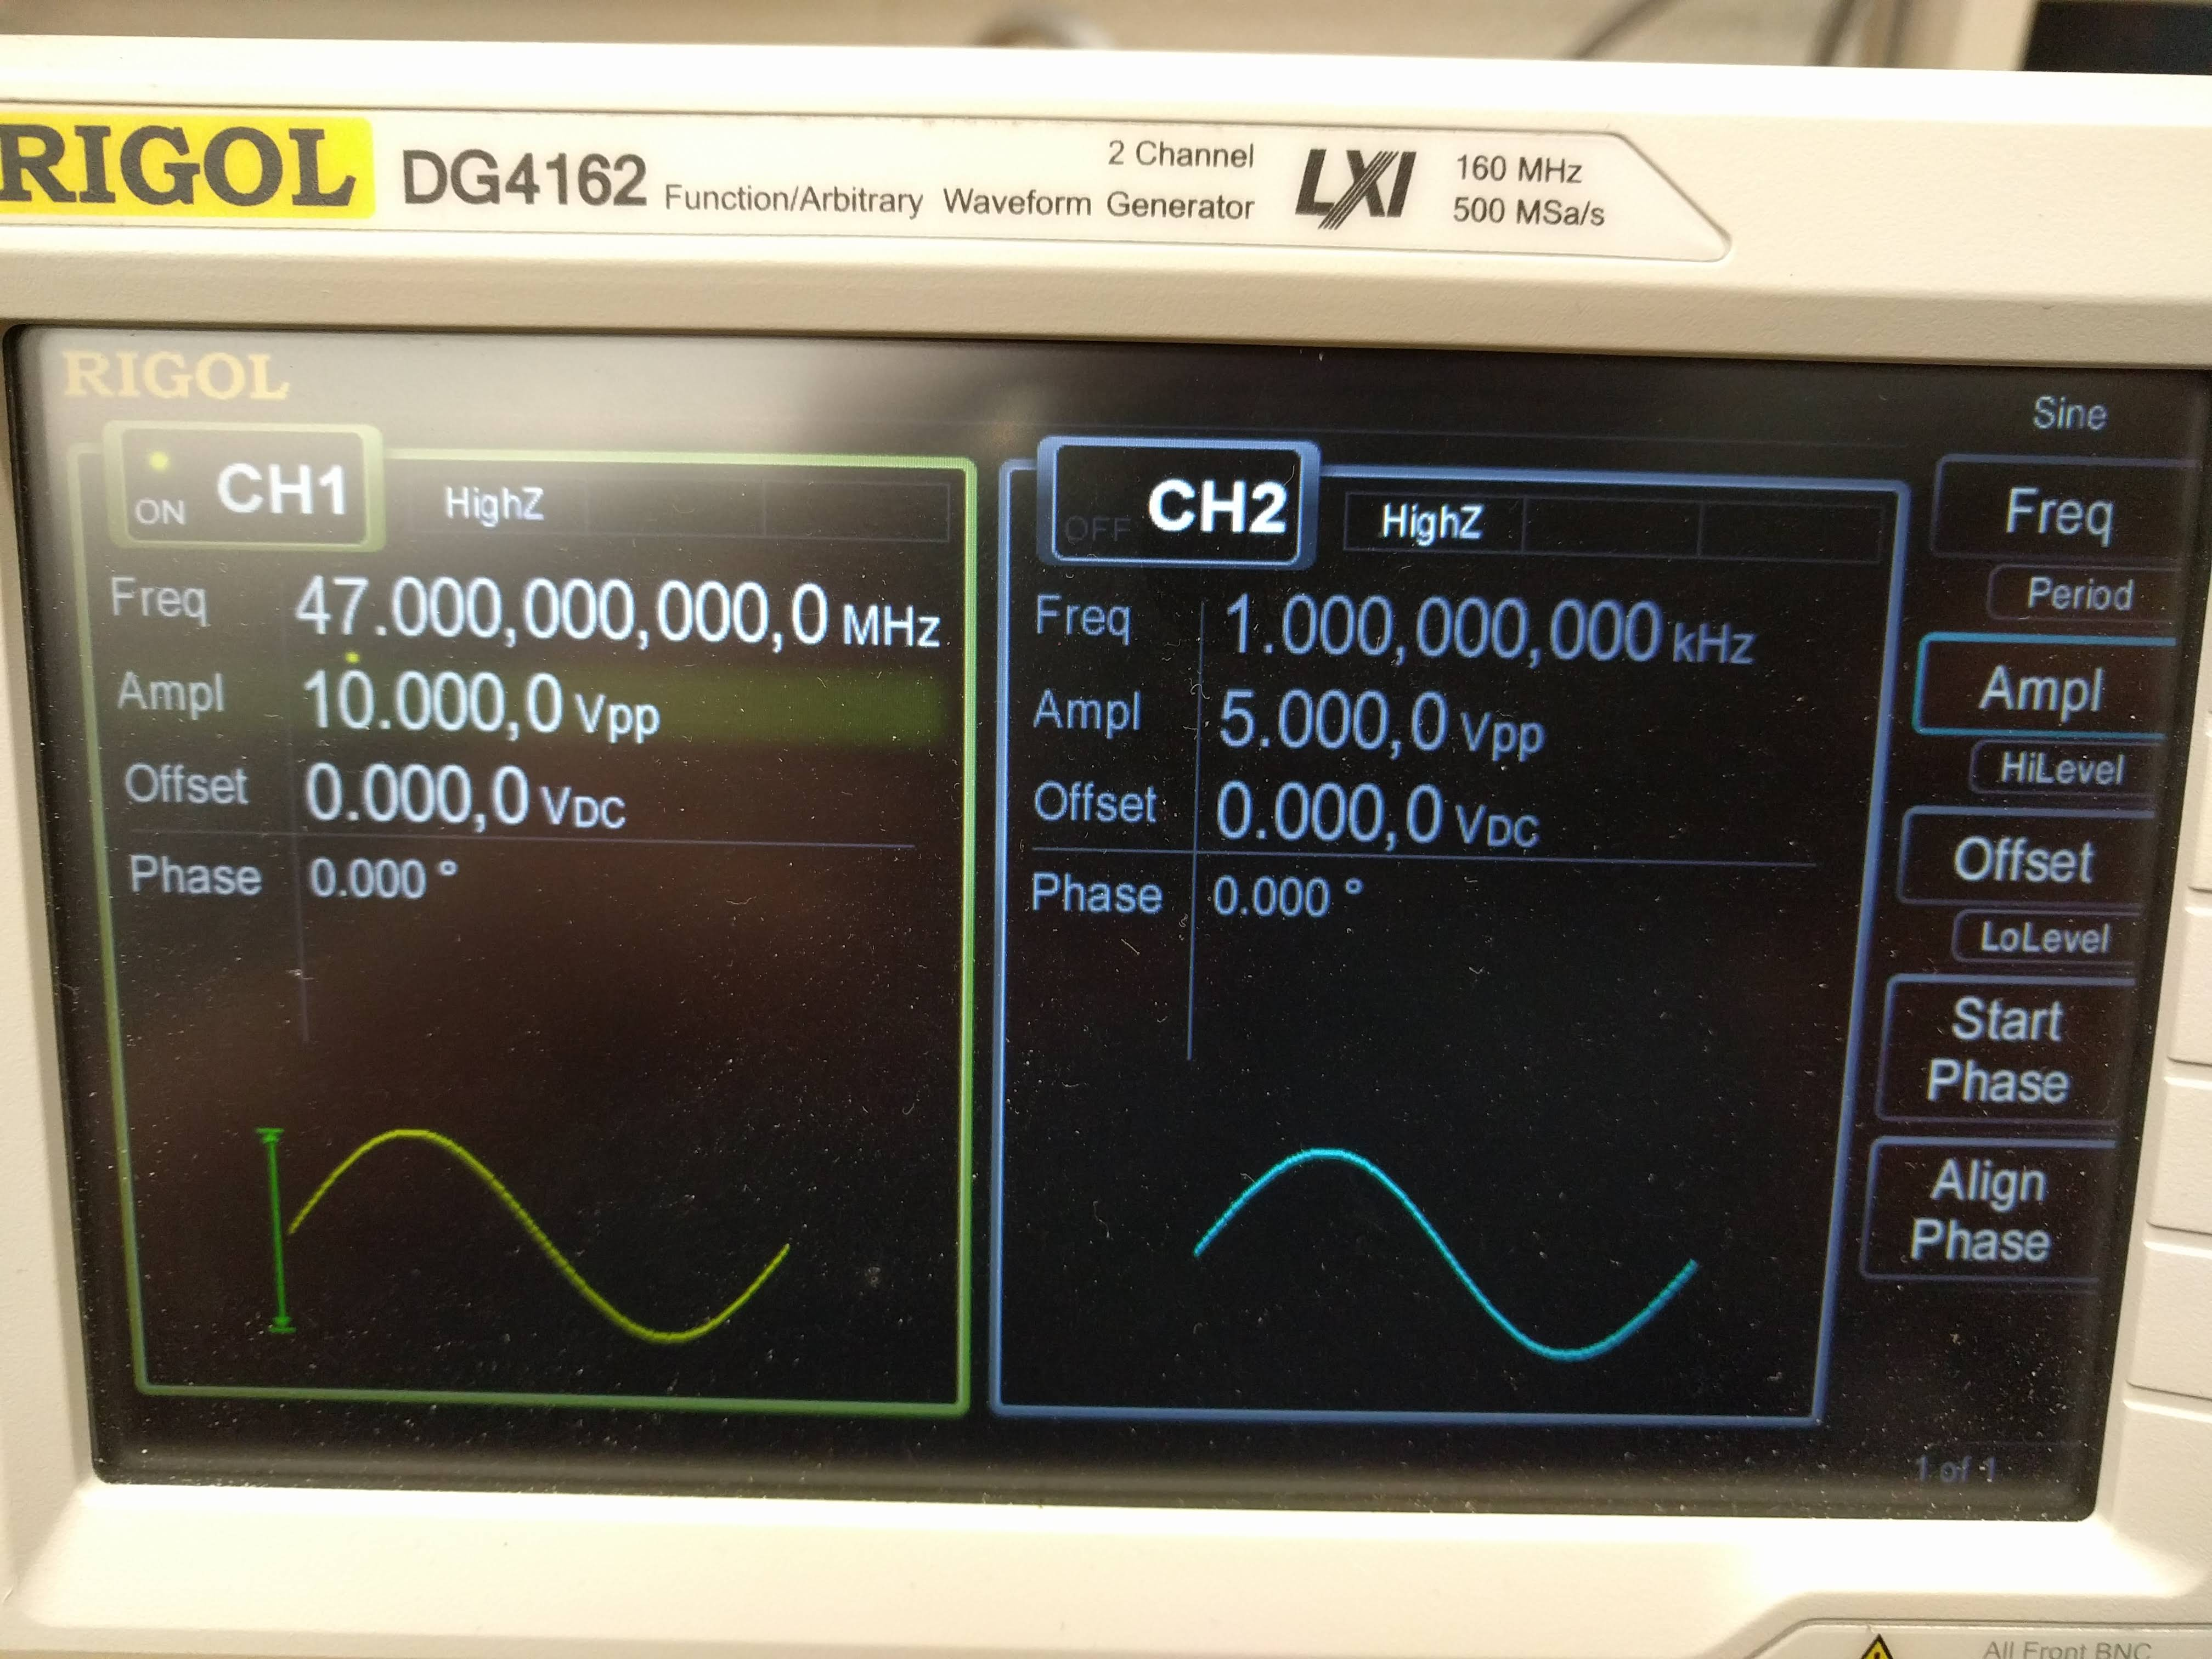
\includegraphics[width=\linewidth]{pictures/47Mhz.jpg}
    \caption{Function Generator Operating at 47MHz}
    \label{fig:47mhz}
\end{figure}
\begin{figure}
    \centering
    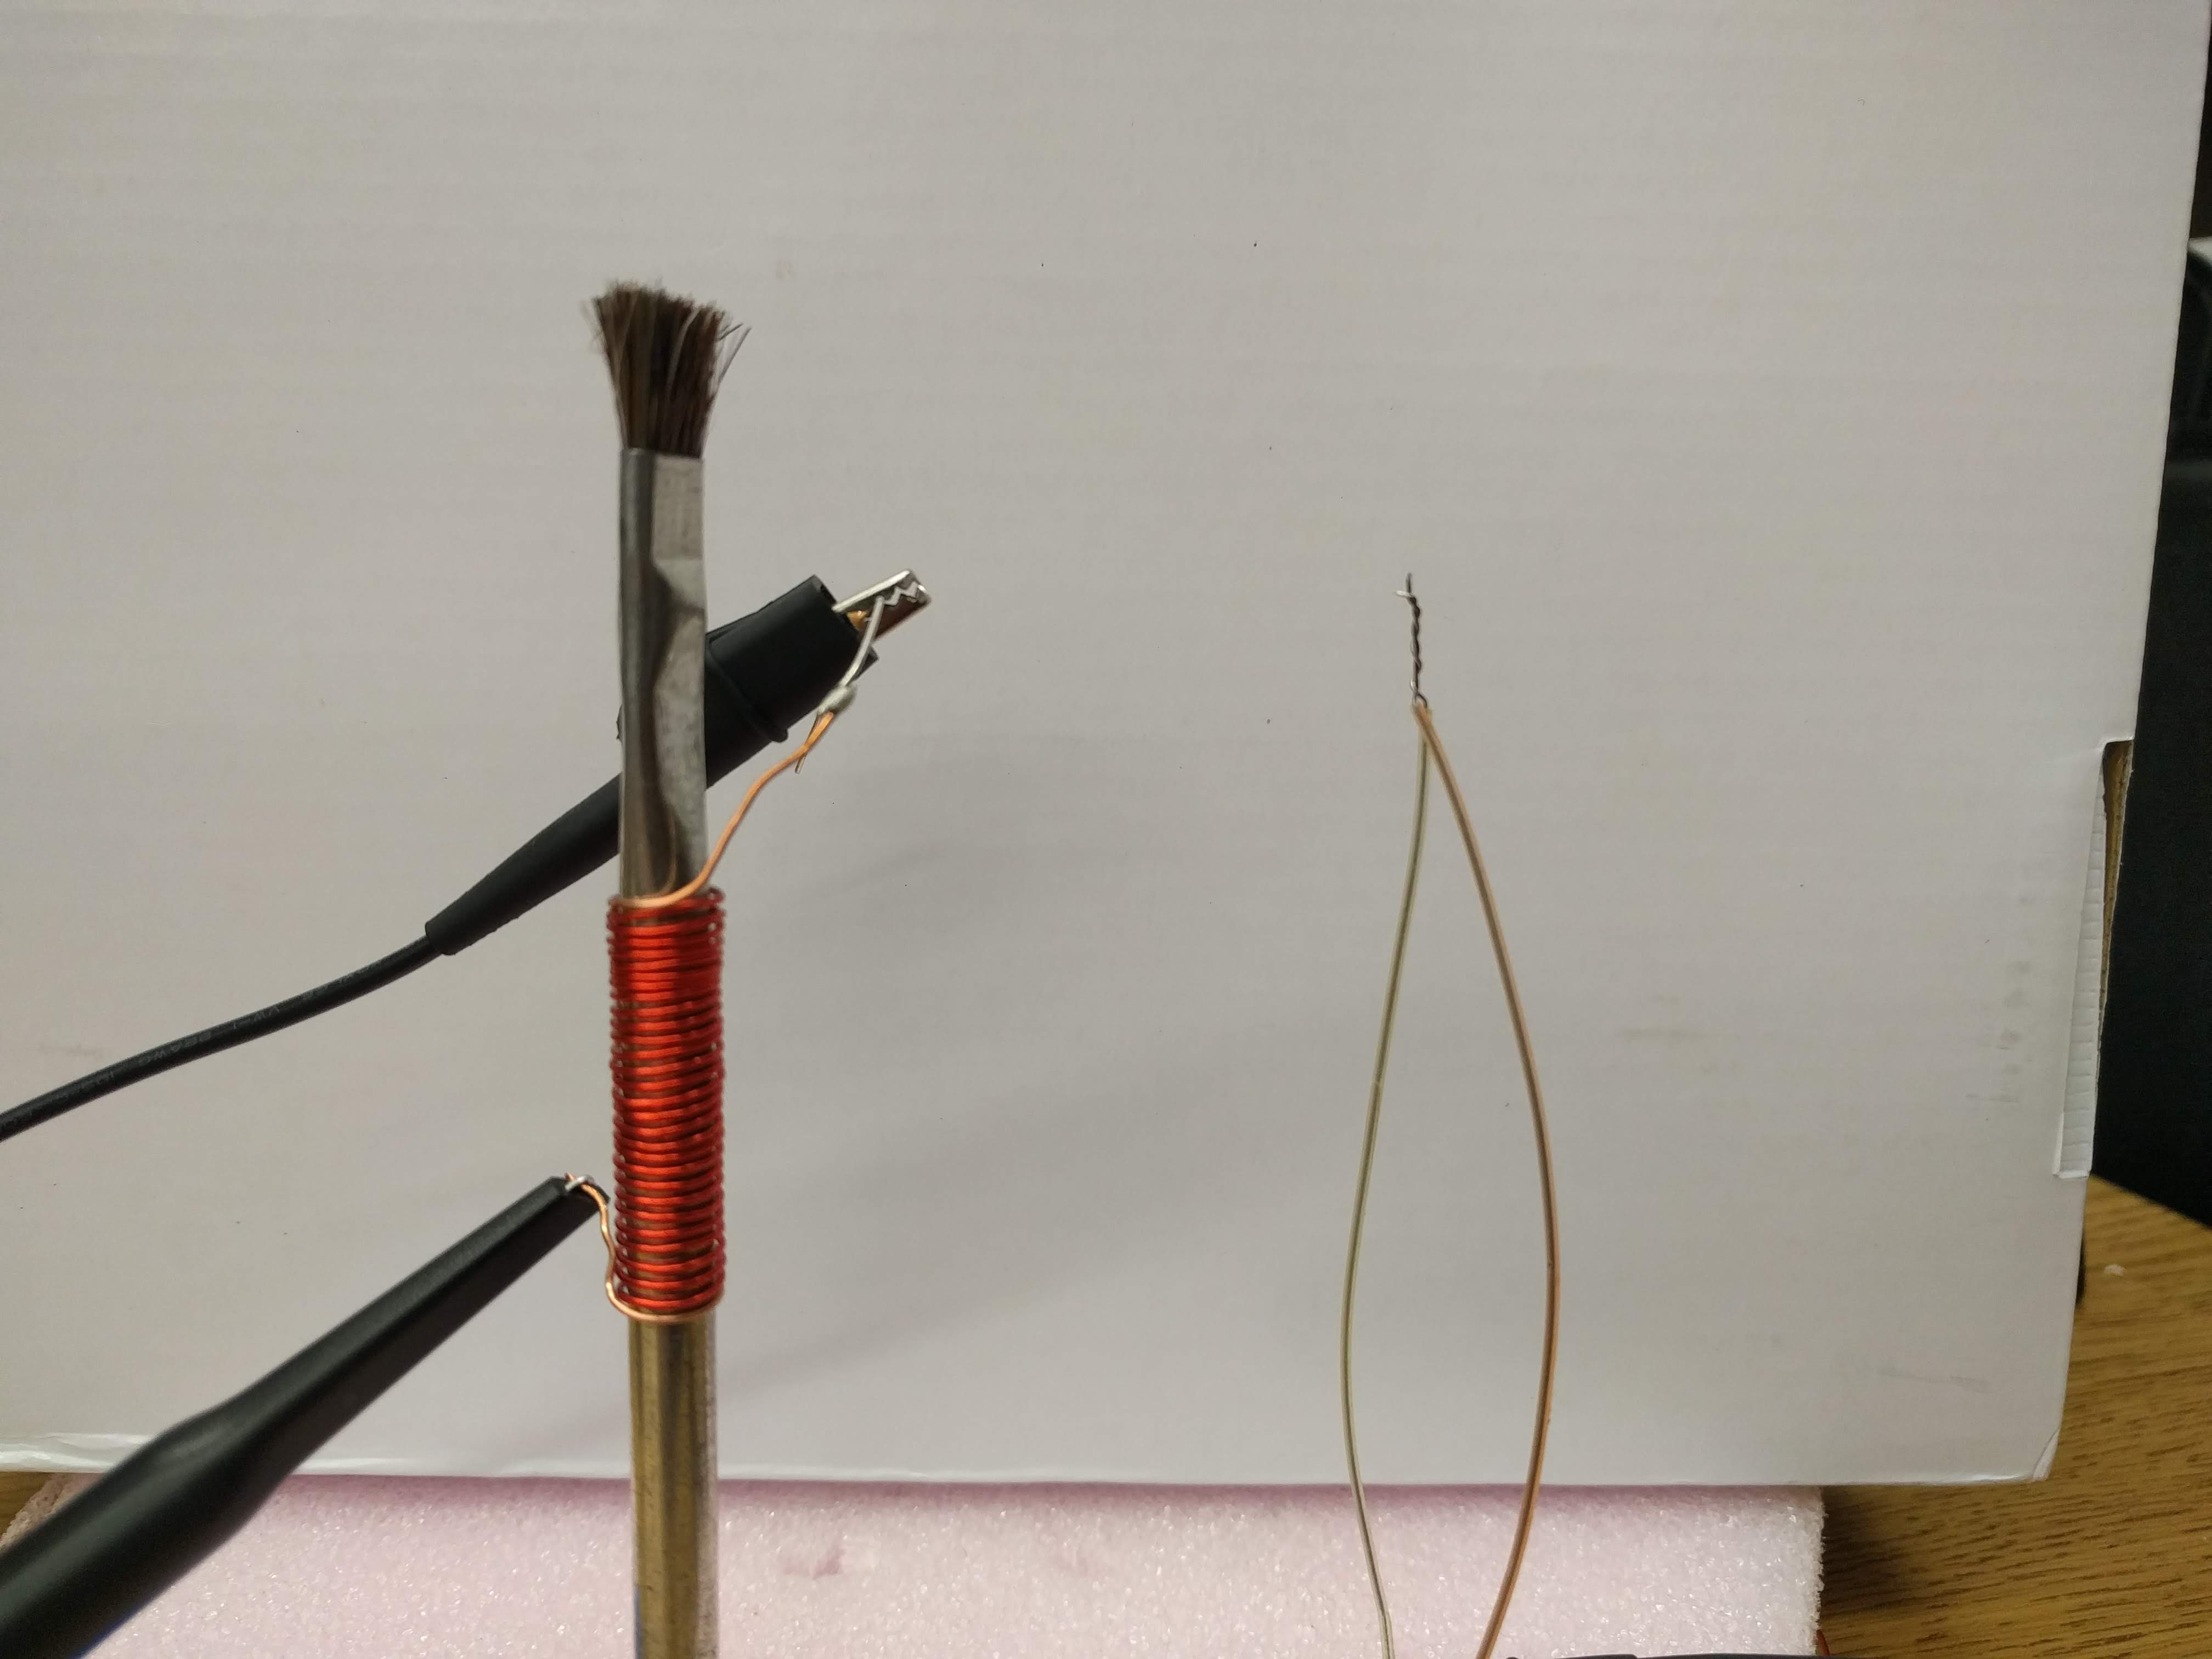
\includegraphics[width=\linewidth]{pictures/Inductor+TCouple.jpg}
    \caption{Inductor and Thermocouple During the Experiment}
    \label{fig:InductorThermocouple}
\end{figure}
\begin{figure}
    \centering
    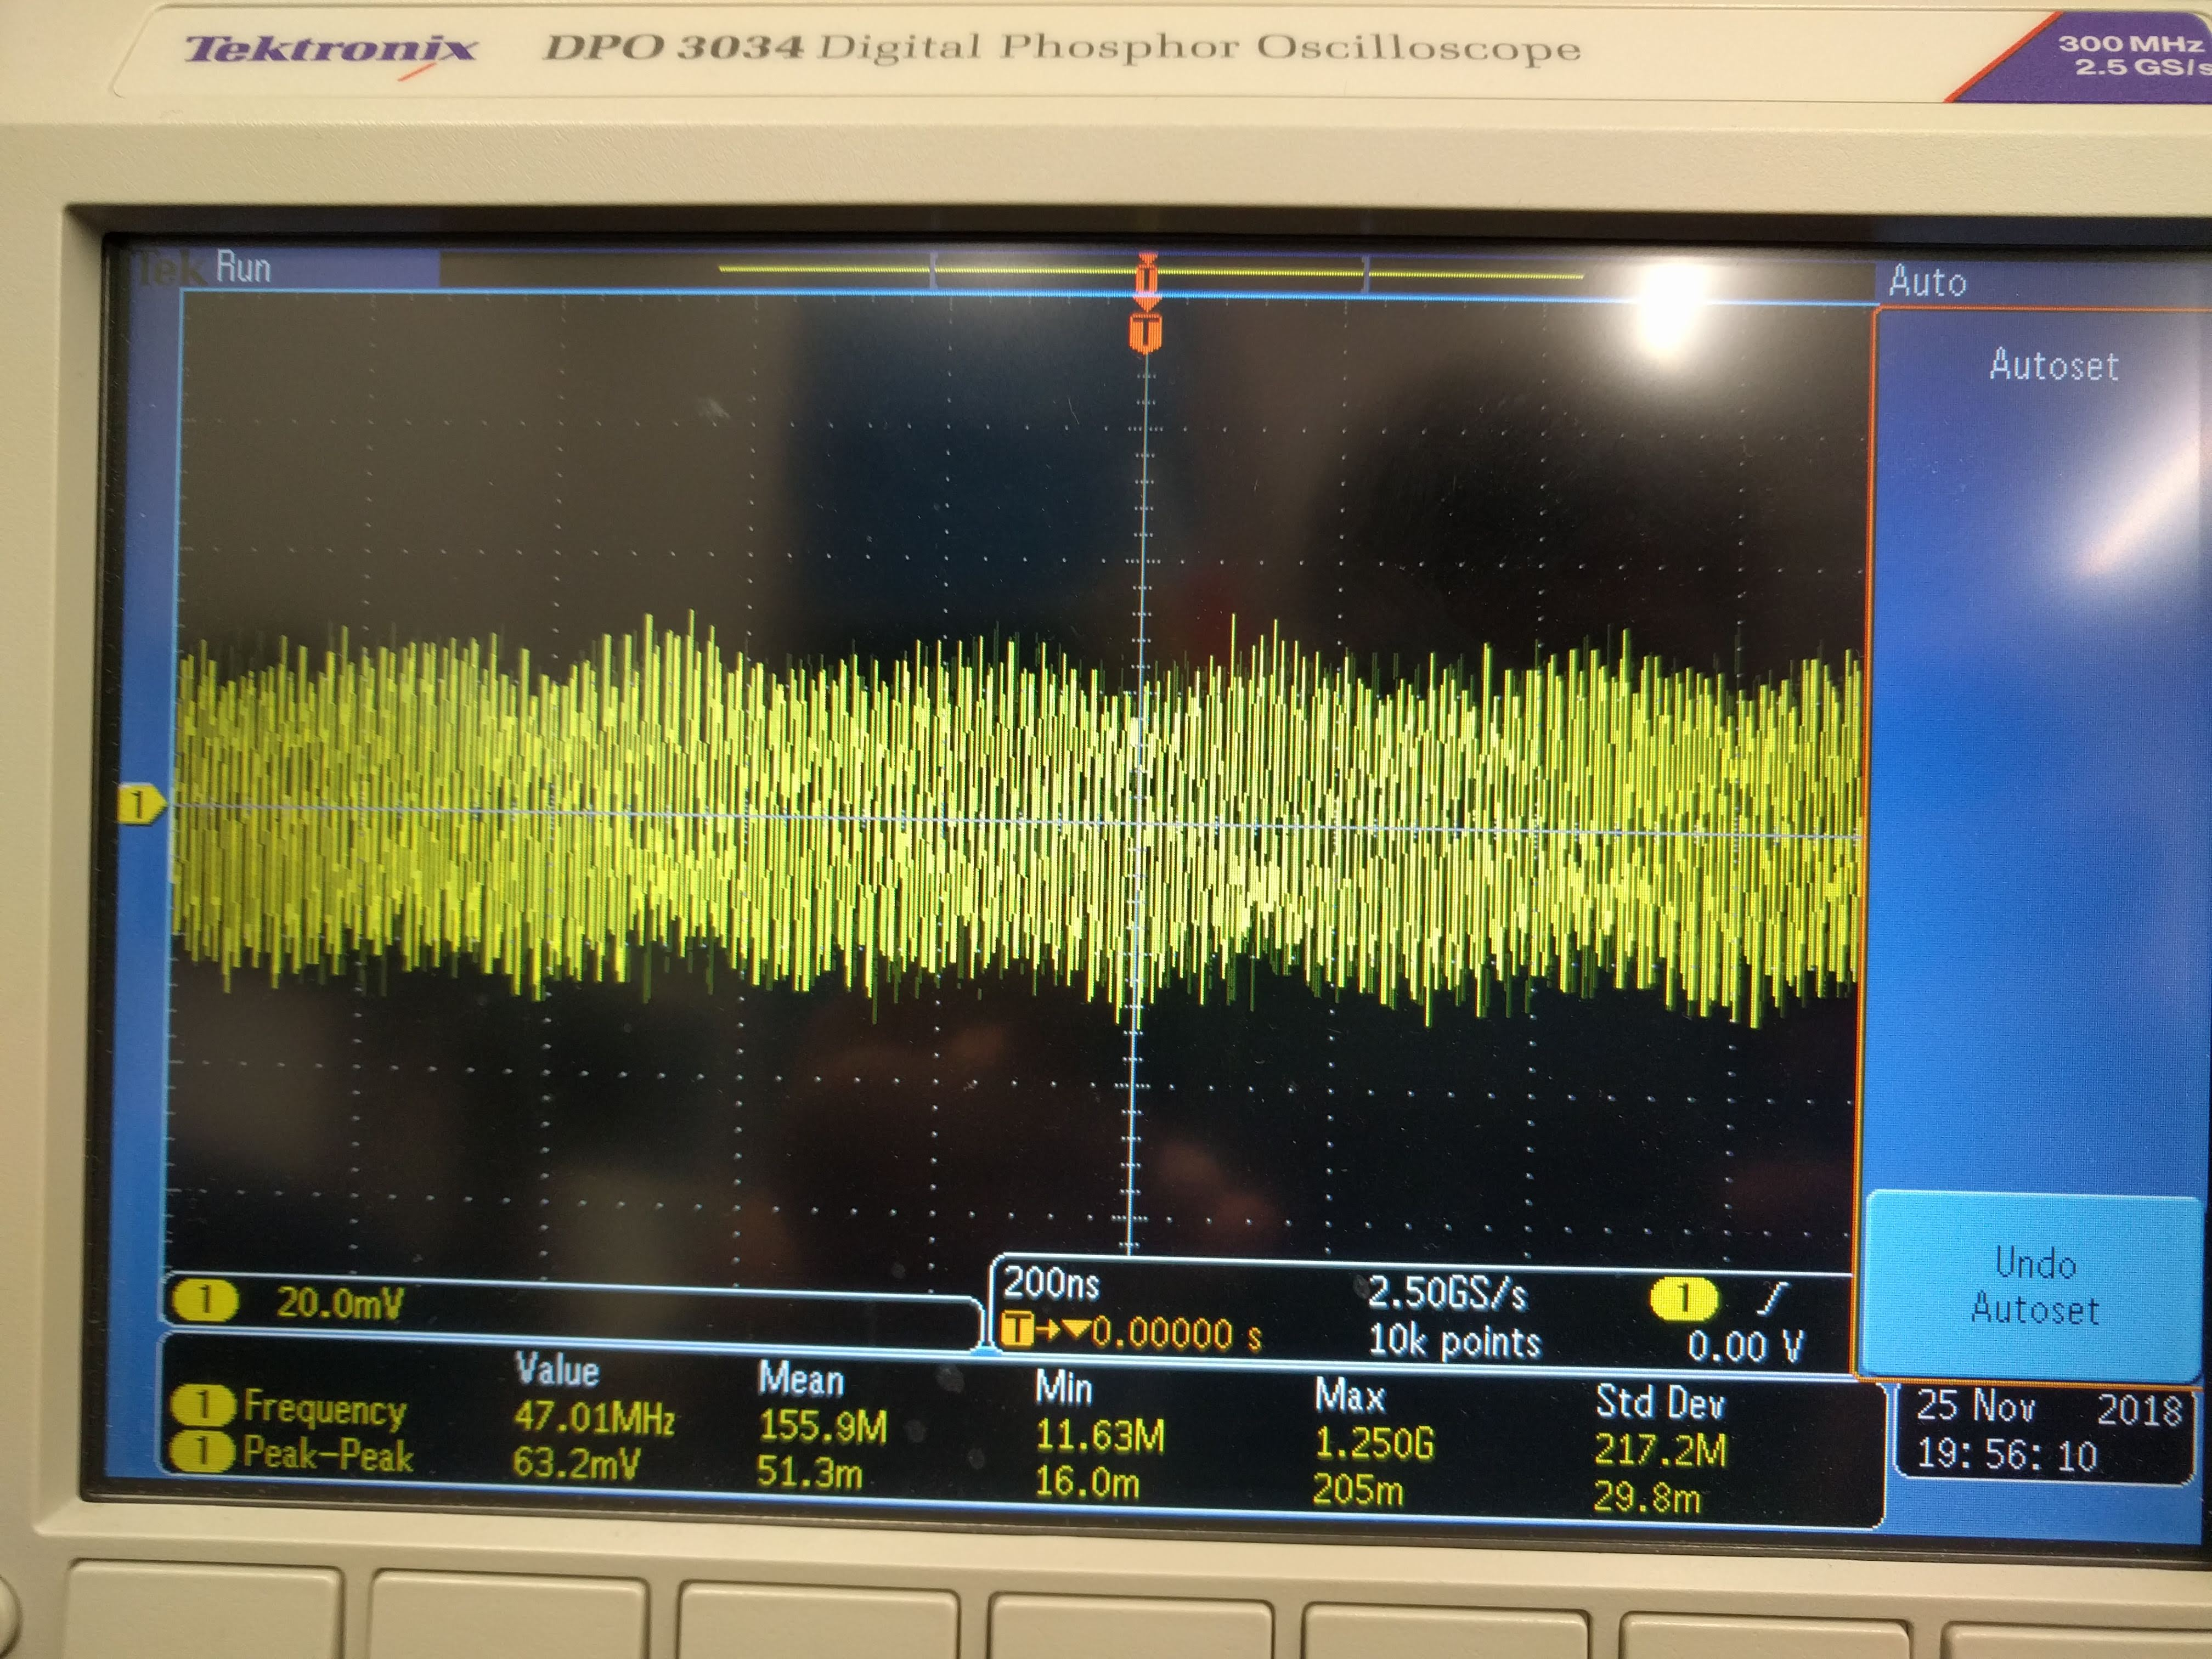
\includegraphics[width=\linewidth]{pictures/Osci-47.jpg}
    \caption{Oscilliscope Showing Induced Waveform}
    \label{fig:Osci47}
\end{figure}
\begin{figure}
    \centering
    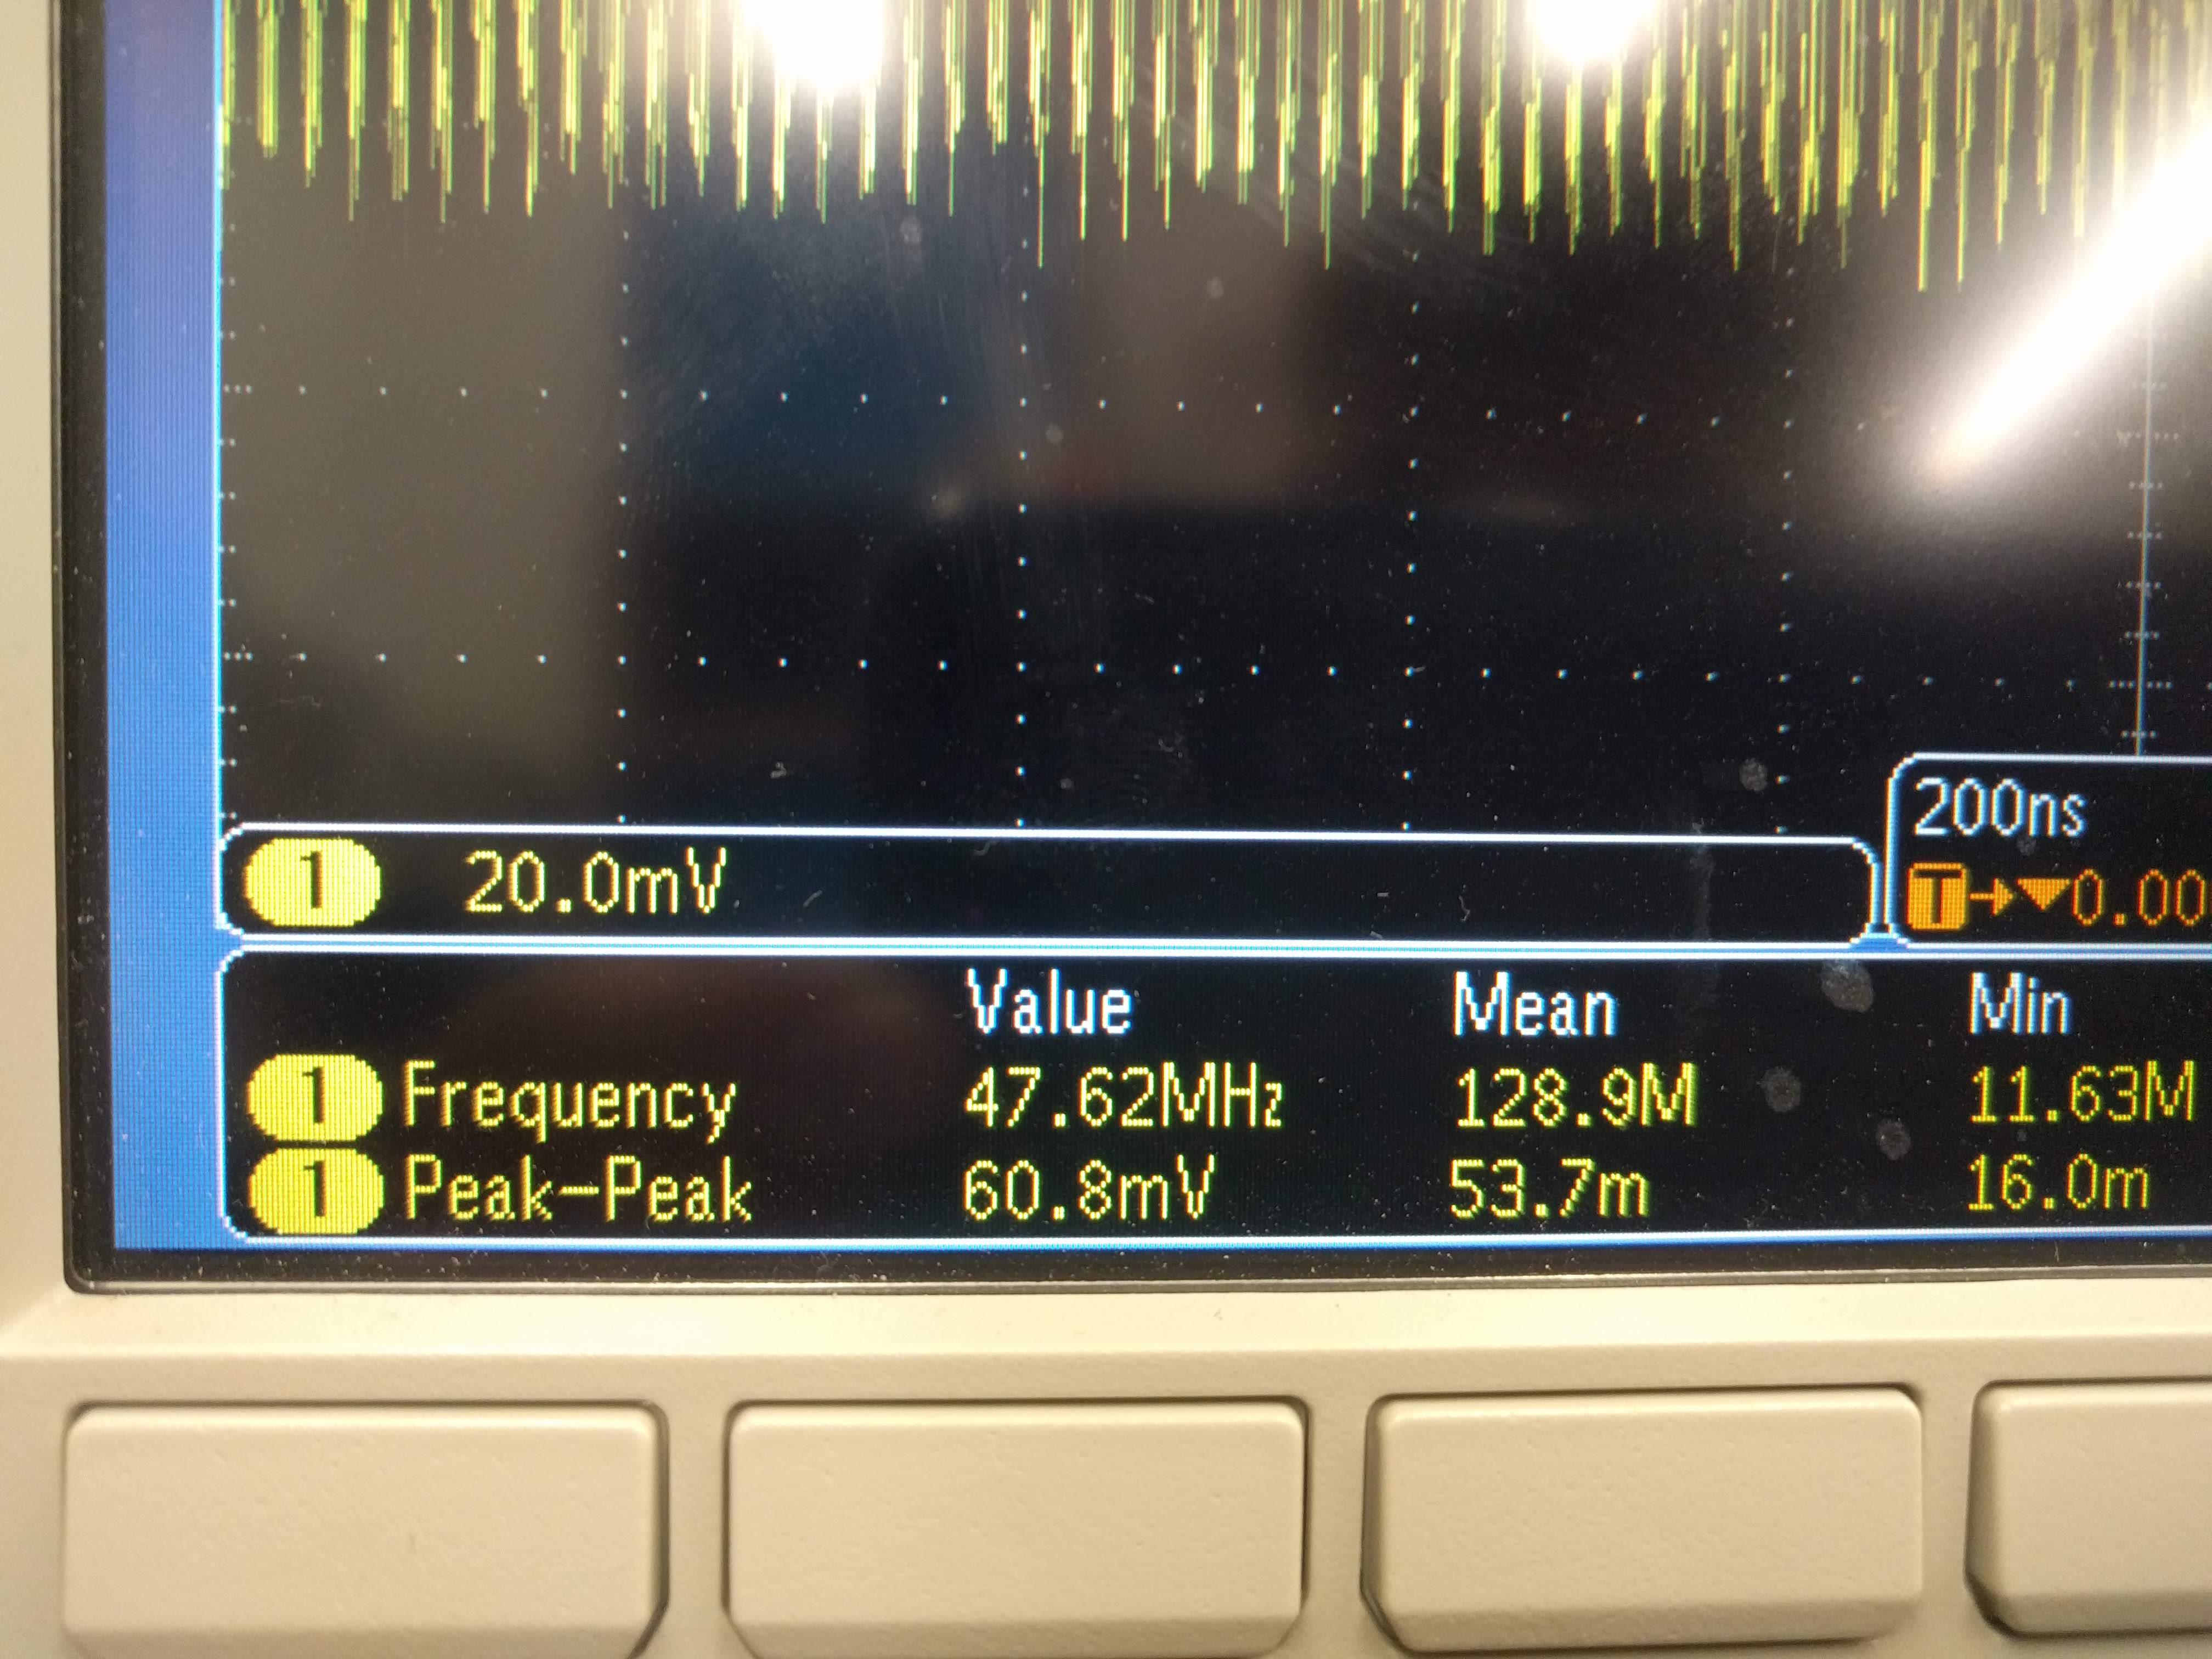
\includegraphics[width=\linewidth]{pictures/Osci-47-2.jpg}
    \caption{47MHz Waveform on Thermocouple}
    \label{fig:Osci47-2}
\end{figure}

The next experiment done was observing the effects of multiple emitters operating at differing frequencies on the thermocouple output. Here, we simply added another inductor connected to the second output of the function generator. We kept the first emitter constant at 47 MHz while stepping the second from 42-52Mhz in increments of 1Mhz. The results were that the induced signal on the thermocouple was the constructive/destructive interference between the two input signals. An example is shown in \cref{fig:fgencombo,fig:InductorThermocoupleCombo,fig:OsciHarmonic}. Once again, the induced signal did not translate to real temperature output interference. Instead, the thermocouple continued to operate normally. 

\begin{figure}
    \centering
    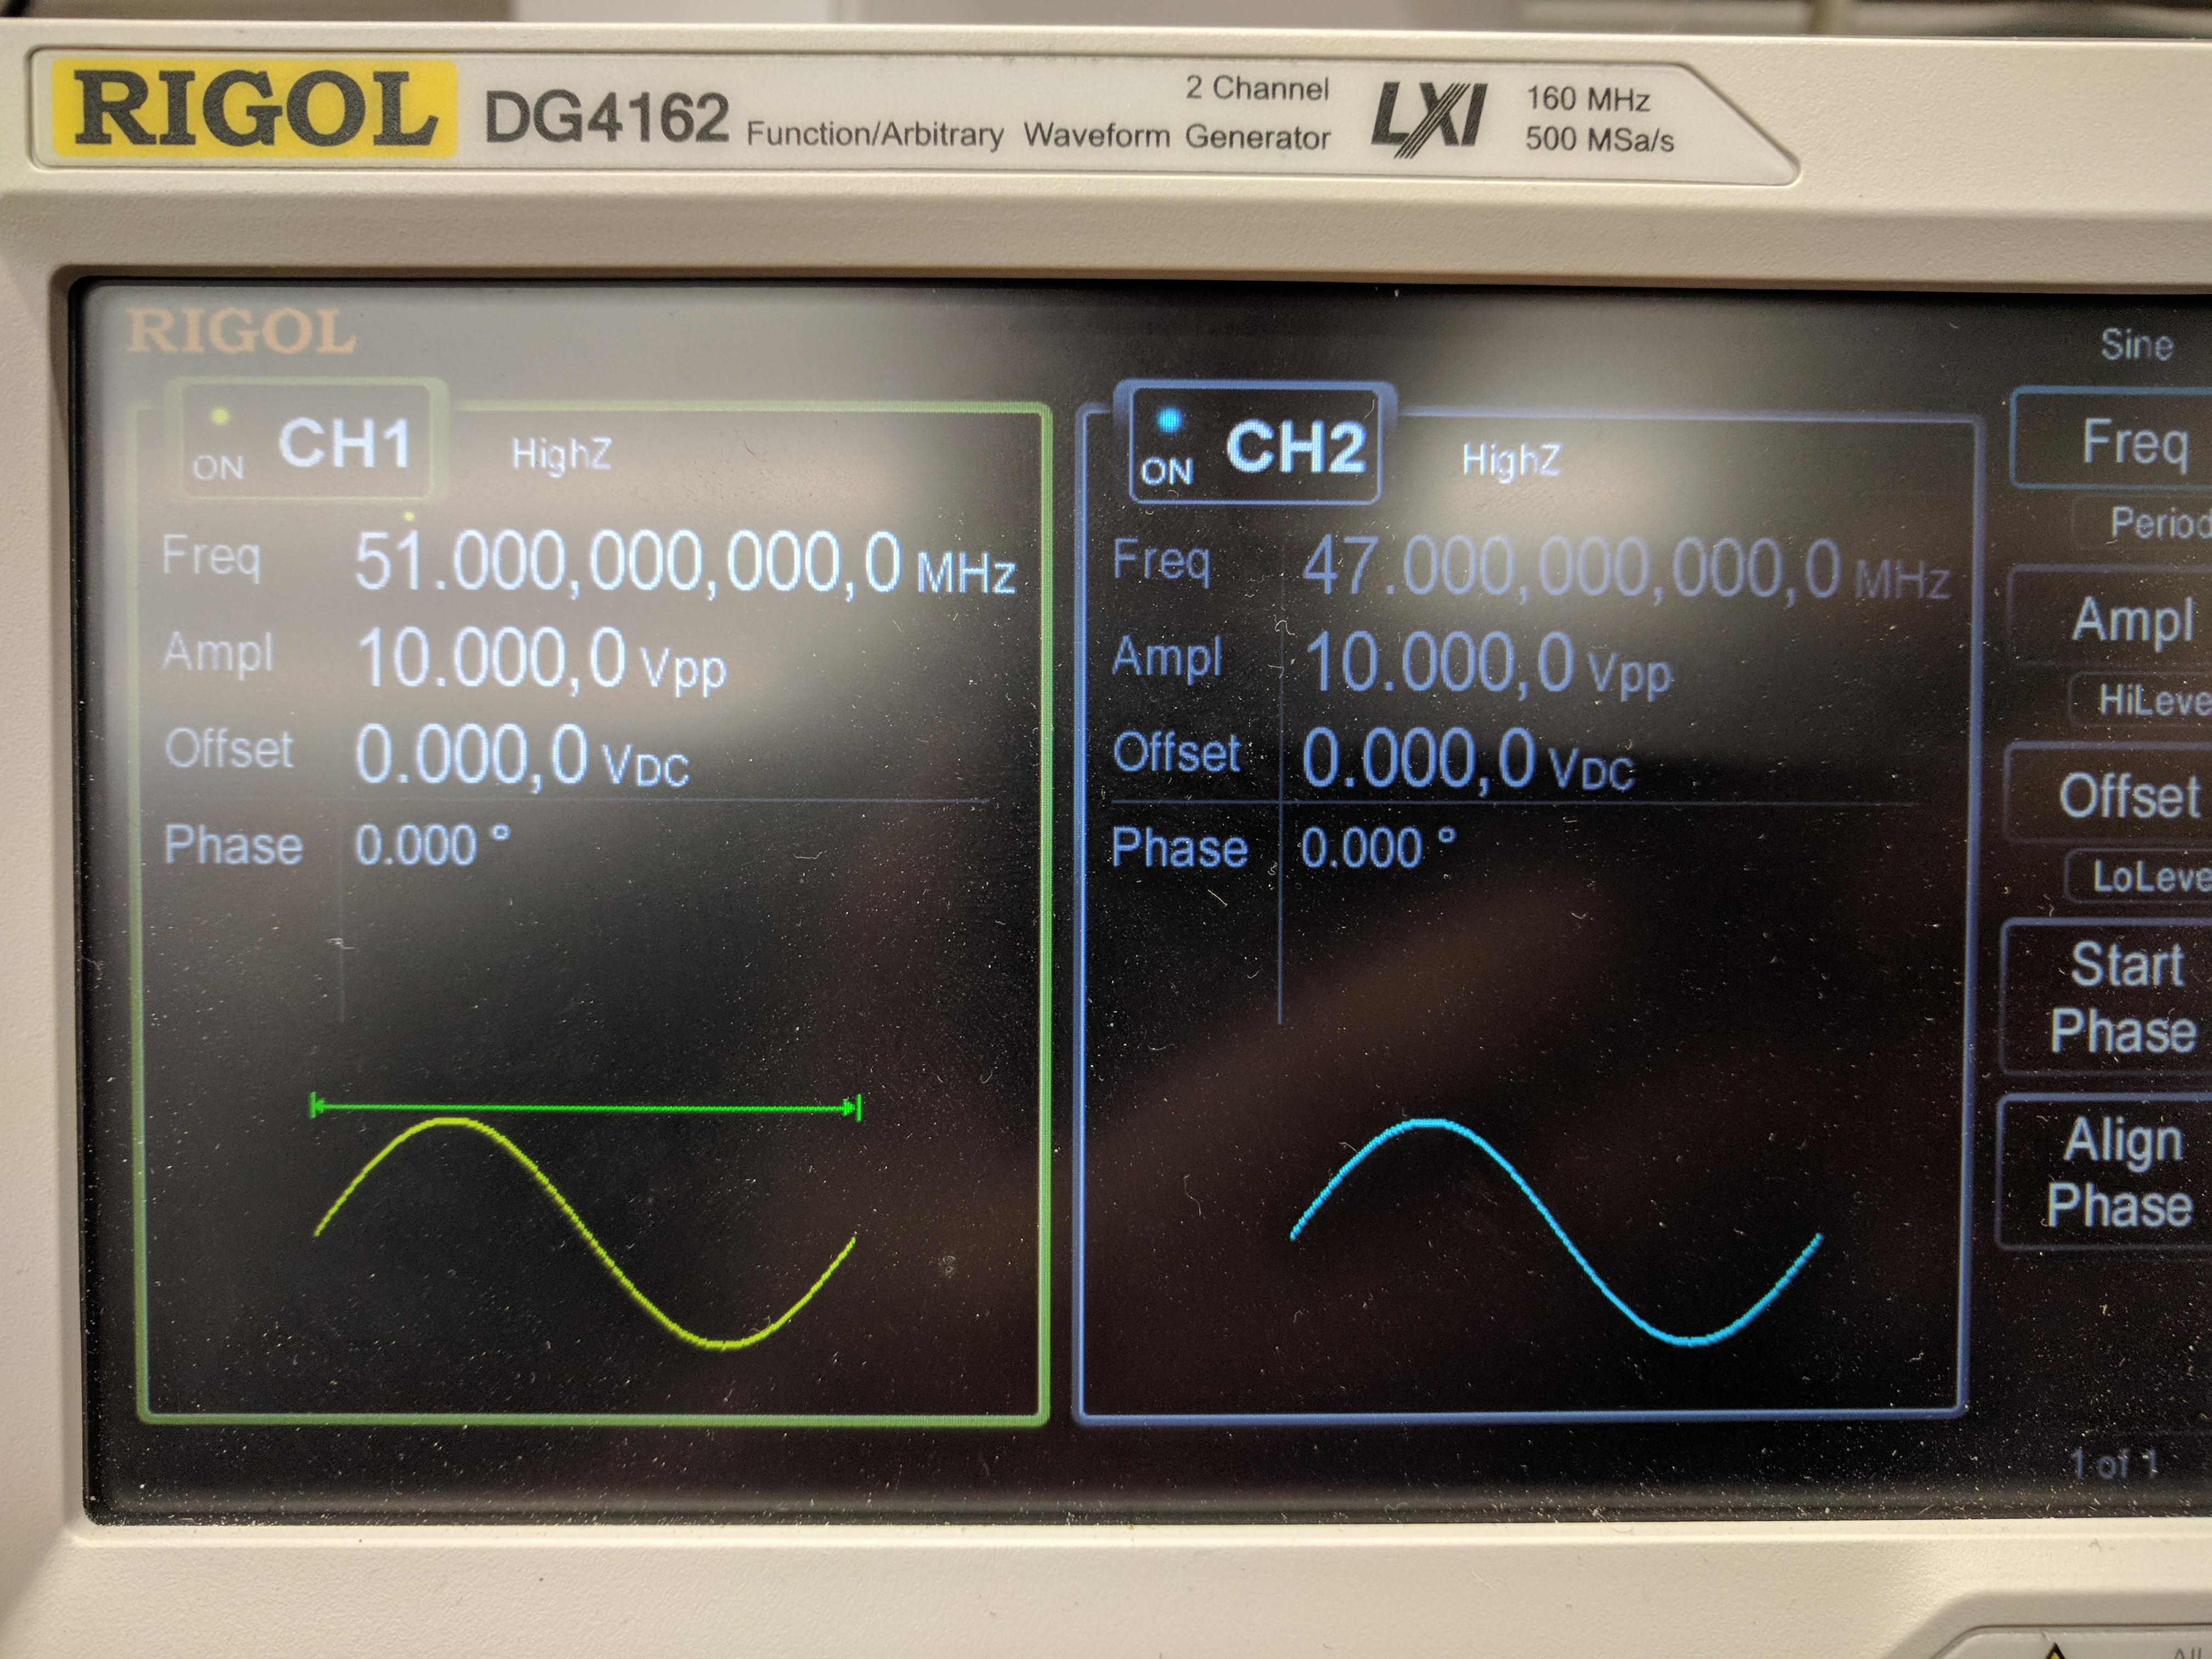
\includegraphics[width=\linewidth]{pictures/FGen-Combo.jpg}
    \caption{Function Generator Operating at Two Frequencies}
    \label{fig:fgencombo}
\end{figure}
\begin{figure}
    \centering
    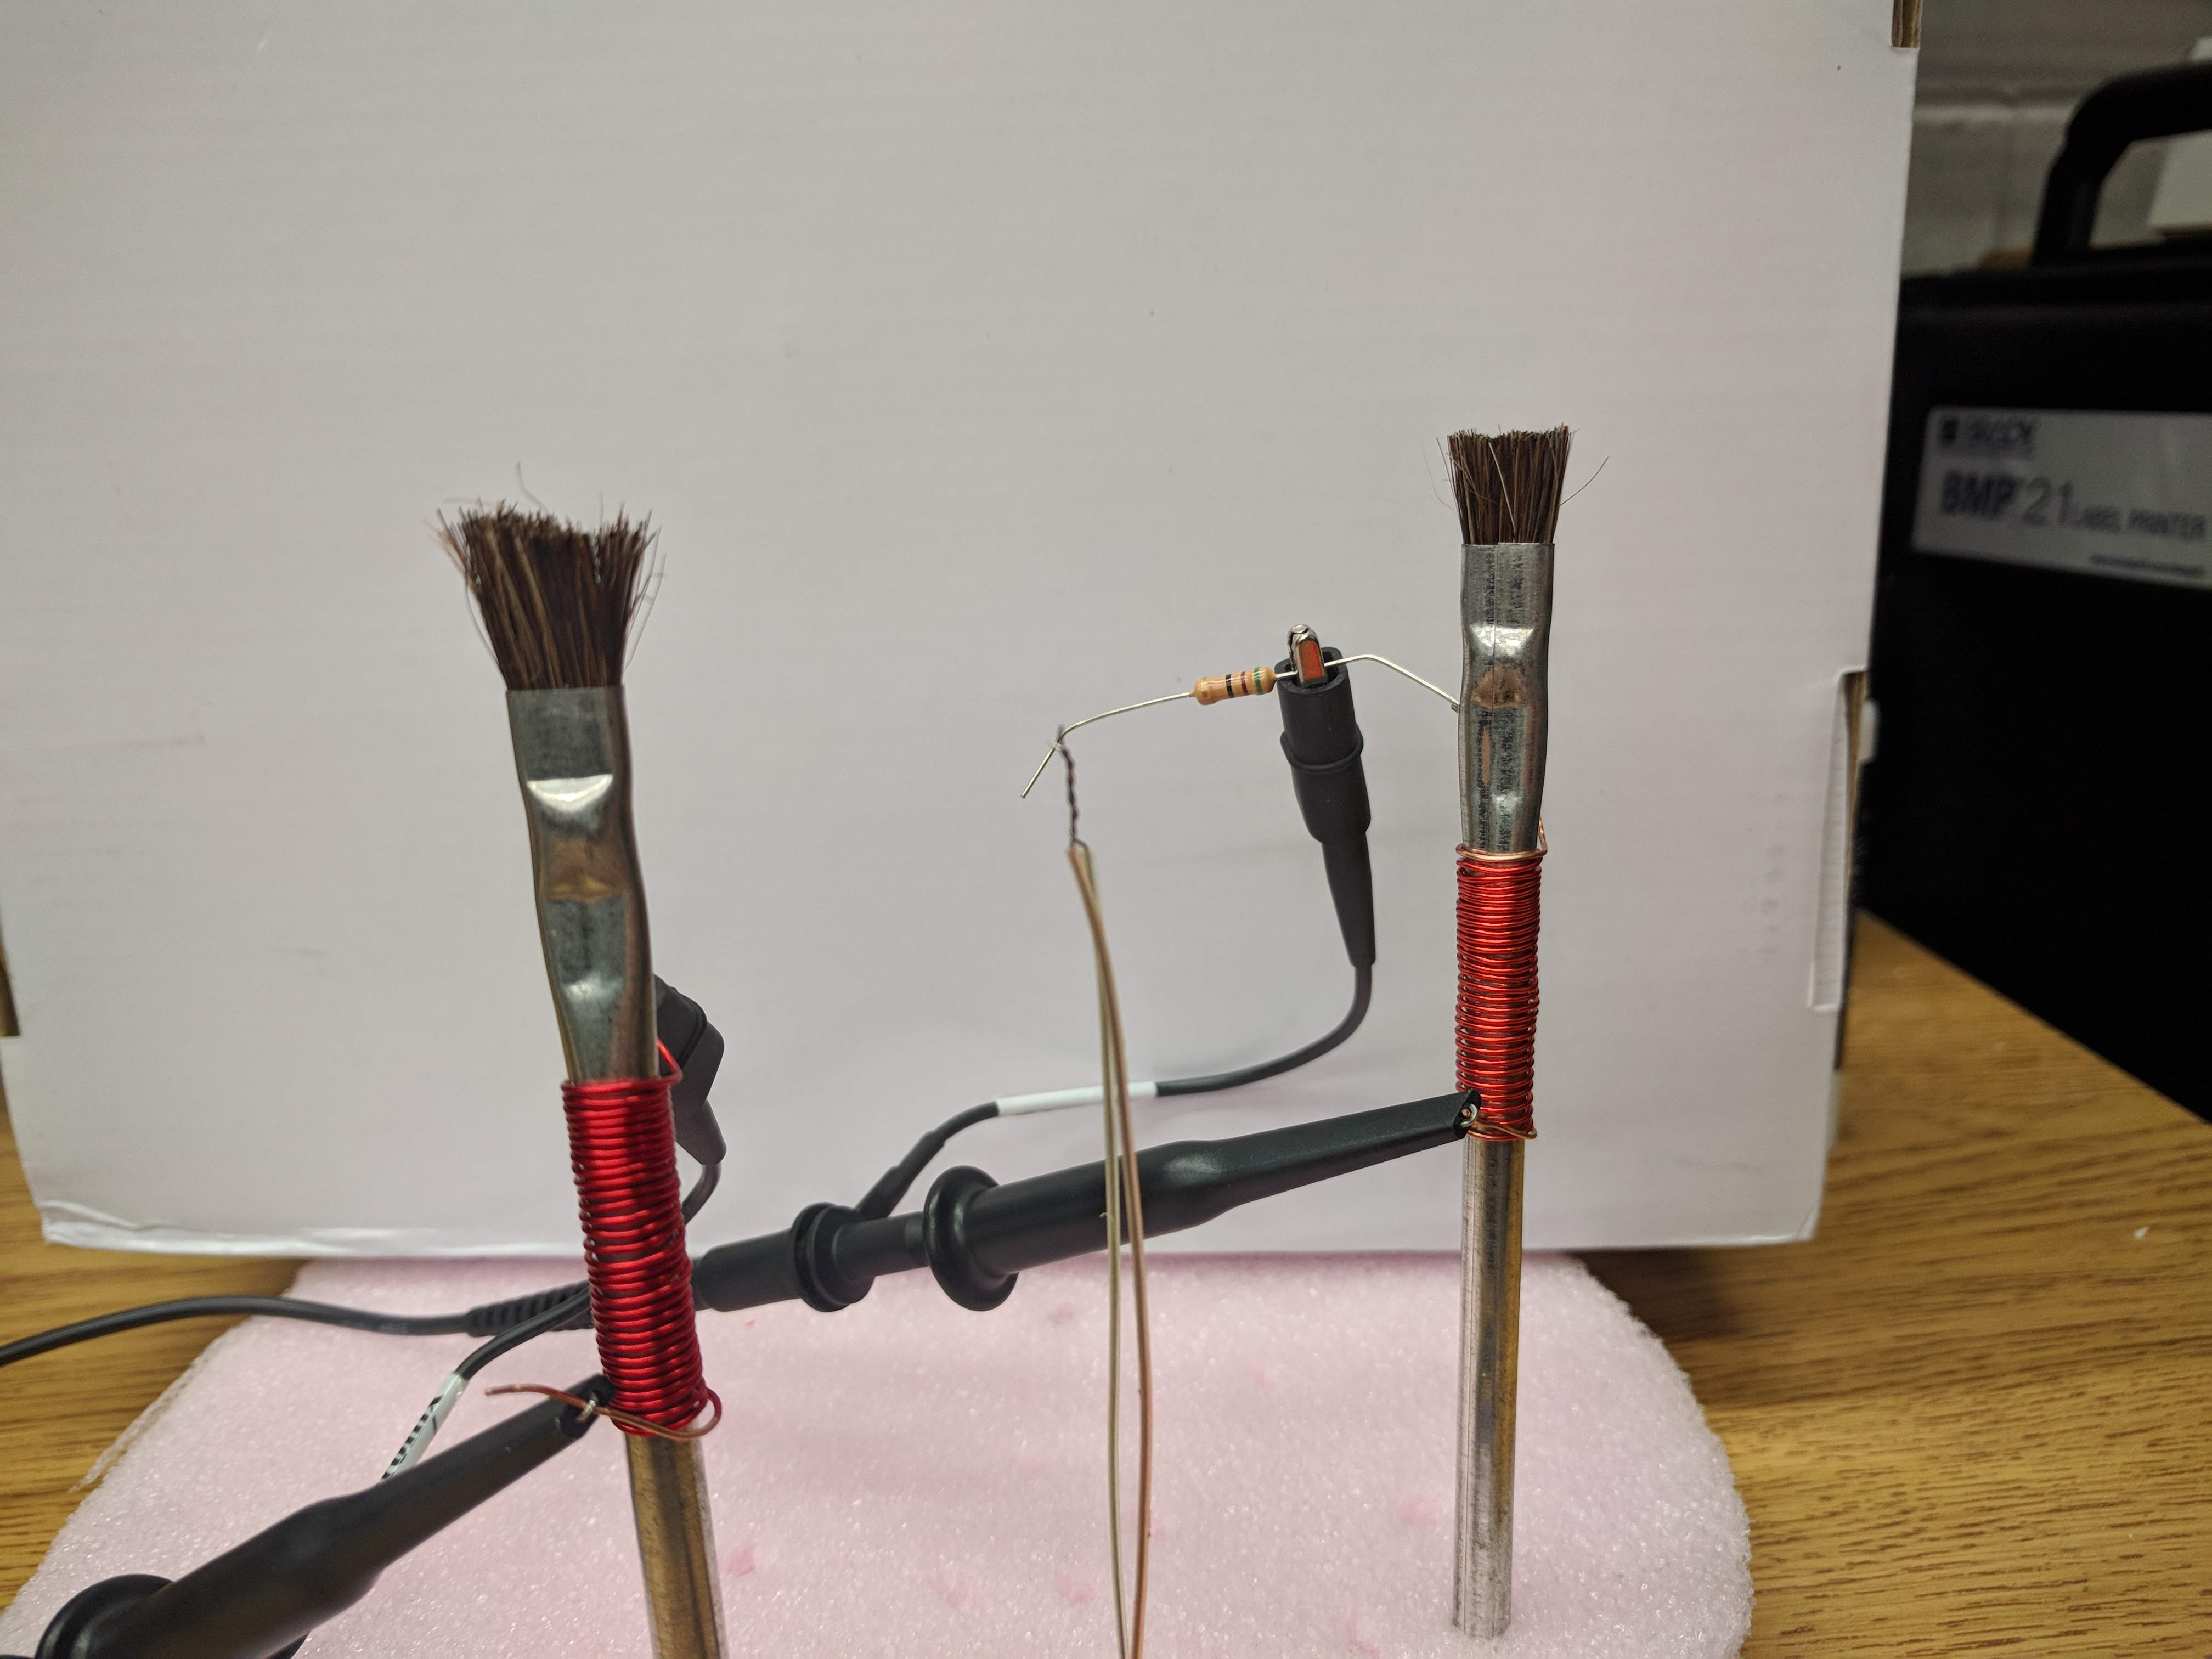
\includegraphics[width=\linewidth]{pictures/Tcouple-Combo.jpg}
    \caption{Inductor and Thermocouples During the Experiment}
    \label{fig:InductorThermocoupleCombo}
\end{figure}
\begin{figure}
    \centering
    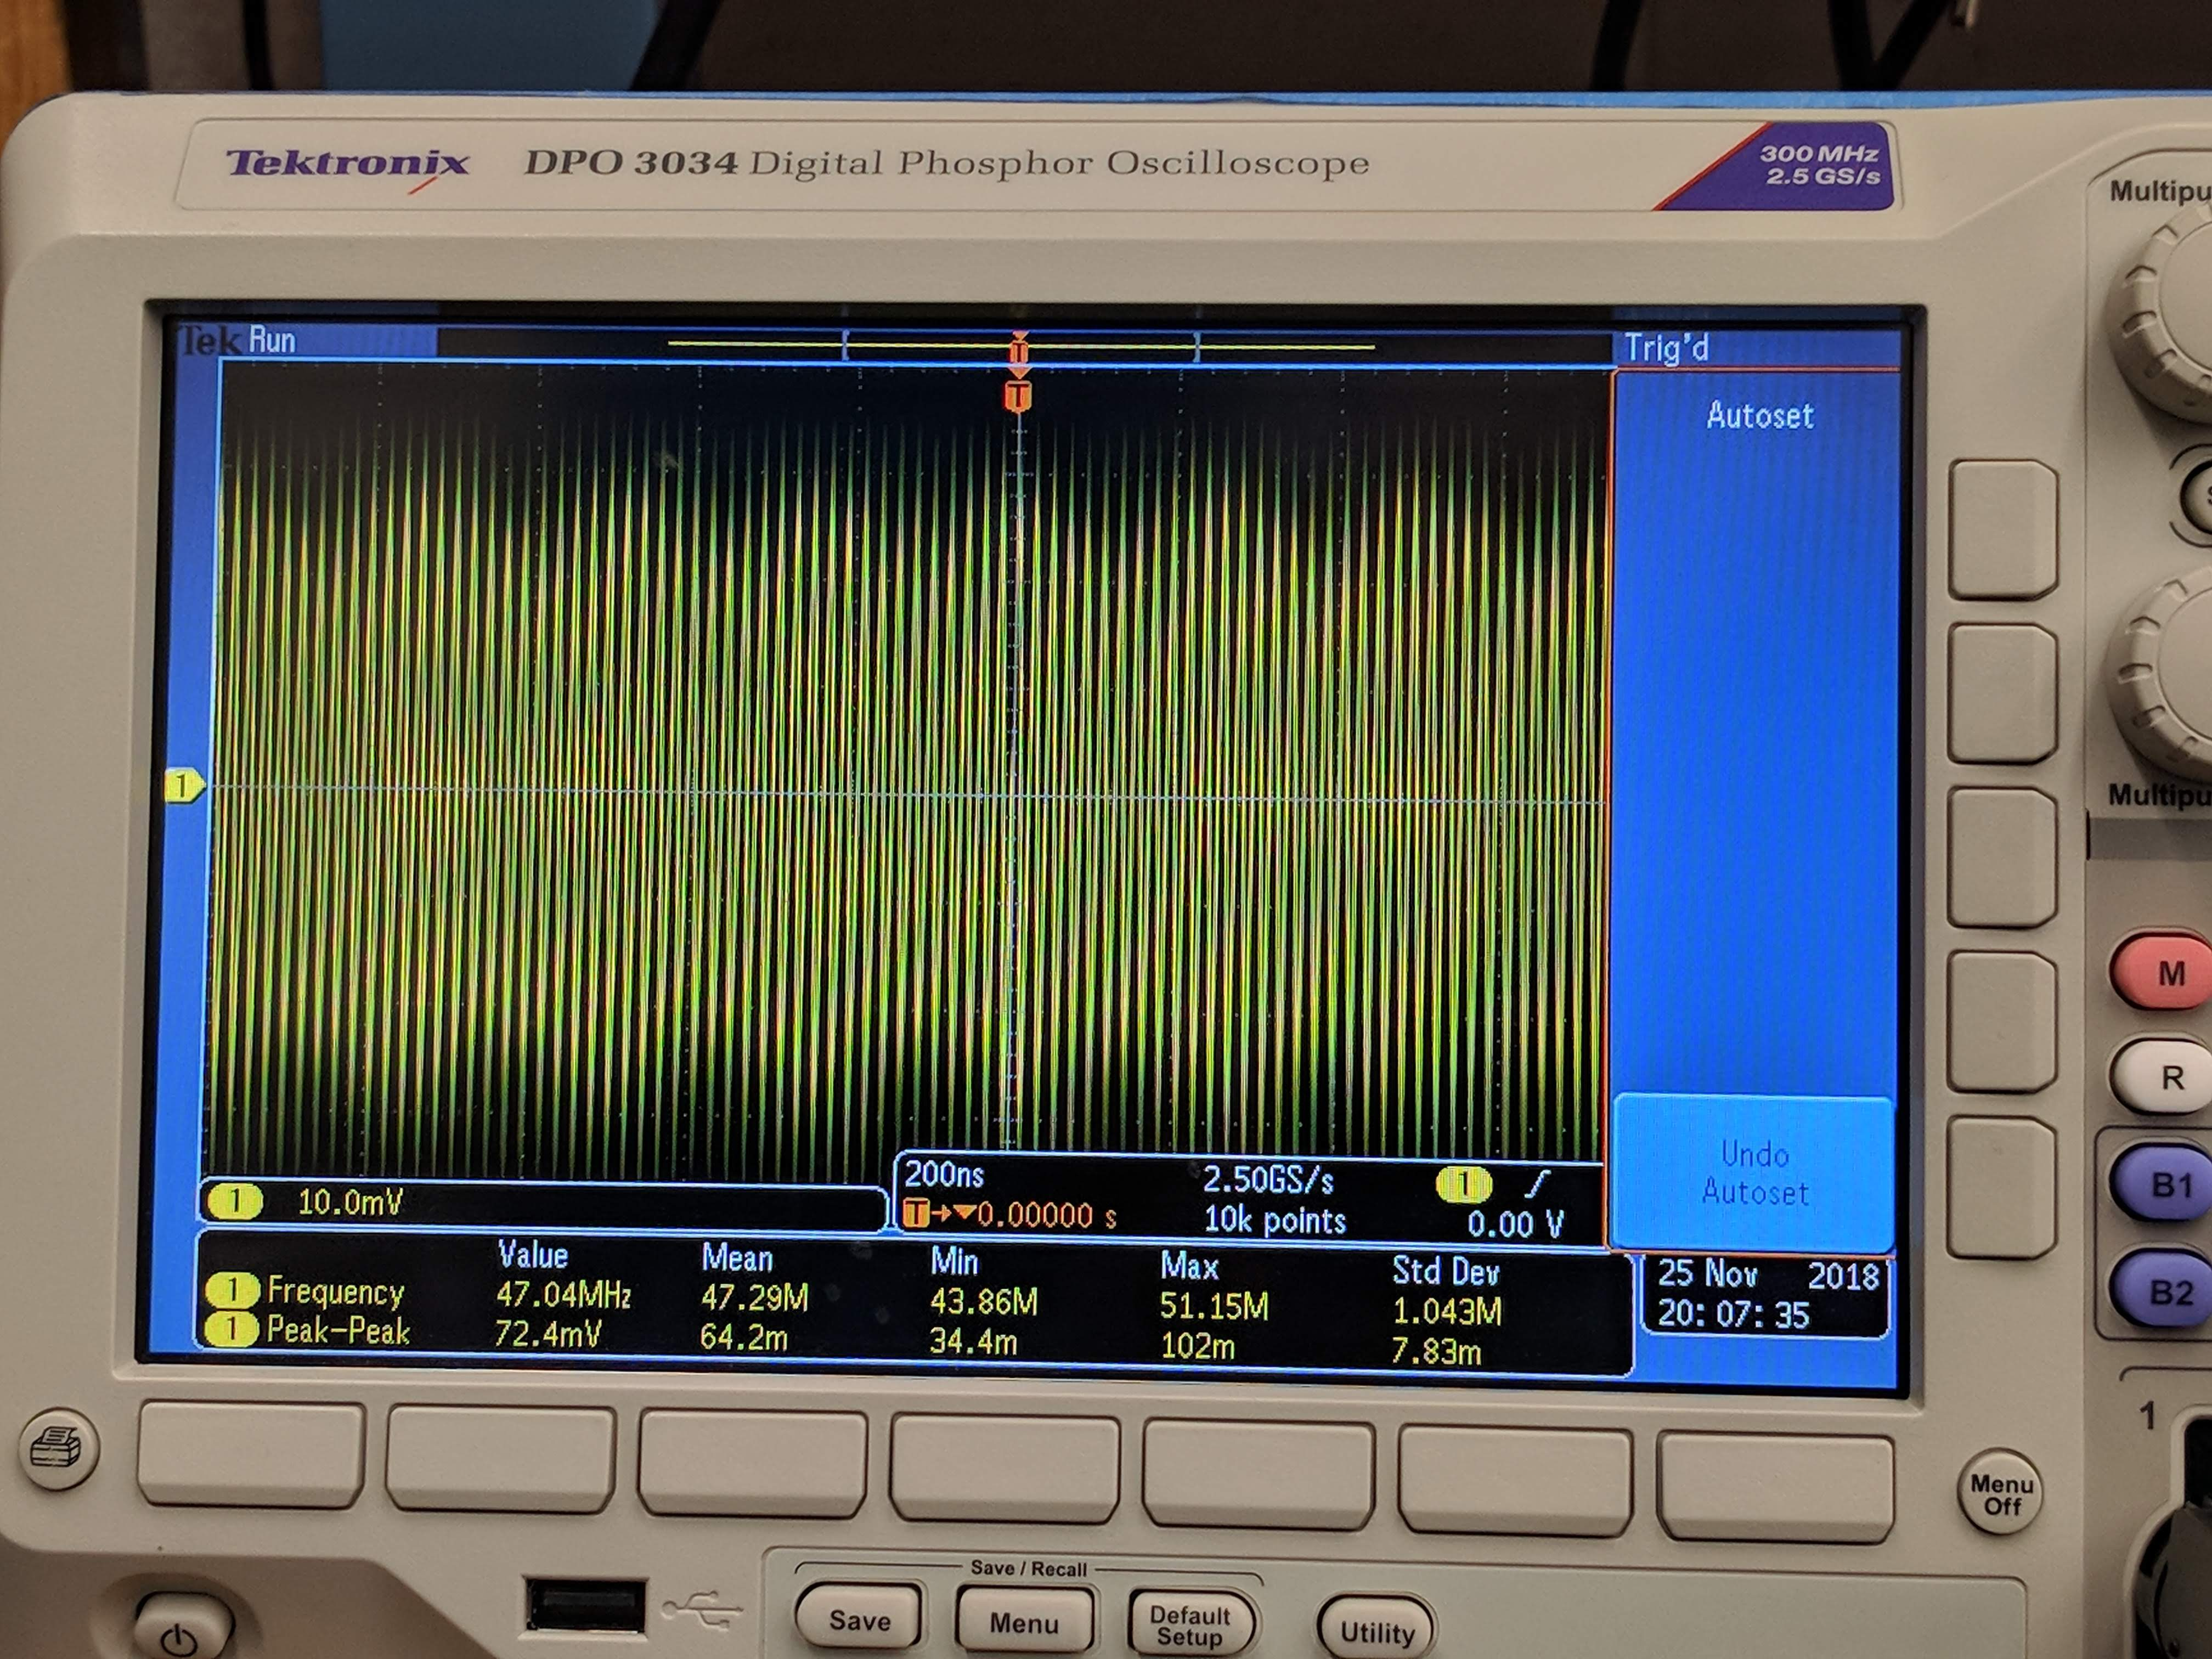
\includegraphics[width=\linewidth]{pictures/Harmonic.jpg}
    \caption{Oscilloscope Showing 47Mhz Harmonic as a Result of Multiple Inductors}
    \label{fig:OsciHarmonic}
\end{figure}

\subsection{What went wrong}\label{wwdw}
From the experiments we were able to learn two things: inducing an \ac{ac} signal on a thermocouple using \ac{emi} is simple at the right frequencies, and that induced signal was not enough to translate to temperature interference. 
On its own, an \ac{ac} signal would not be enough to change the output temperature. This is because the mean value of any sine wave is zero. So, no change in what the MAX31856 was measuring would be seen without some \ac{dc} offset being produced. However, the induced signals from the experiments never had a \ac{dc} offset, thus explaining the lack of interference. 

Another aspect of creating a \ac{dc} offset is that all wires (including the thermocouple itself) have an intrinsic capacitive component. This can result in a rectifier that can convert the induced \ac{ac} signal to a constant \ac{dc} value. In the case of the MAX31856, three additional capacitors are added to the circuit which are meant to reduce noise across the thermocouple wires. A SPICE model derived from the MAX31856 datasheet is shown in \cref{fig:SPICE}. The 0.735V on T- is a result of a bias output from the MAX31856, while V1 is a model of the induced signal on the thermocouple. After a transient simulation \cref{fig:SIM}, the amplitude of the induced signal was reduced to ~70 $\mu V_{pp}$ with no \ac{dc} offset, not appropriate for creating a faulty temperature.  

\begin{figure}
    \centering
    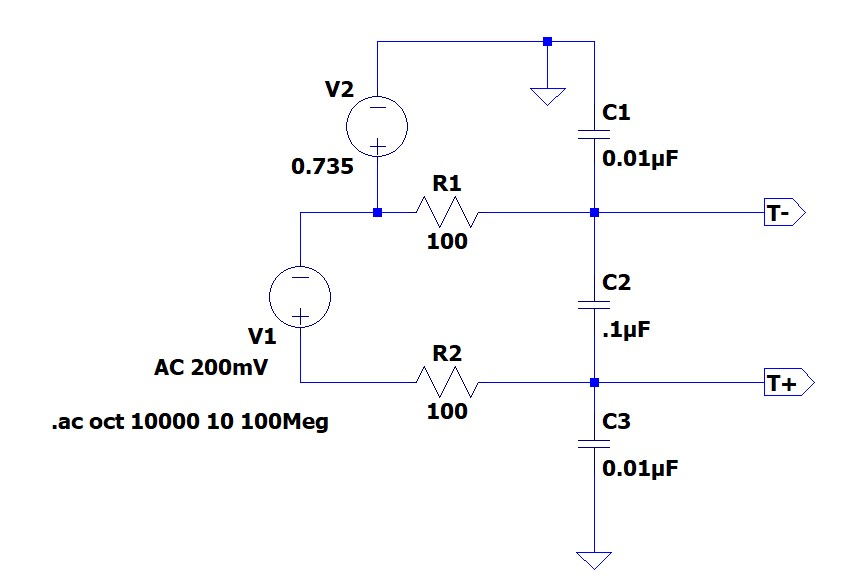
\includegraphics[width=\linewidth]{pictures/SPICE.jpg}
    \caption{SPICE Model of the MAX31856 Interface}
    \label{fig:SPICE}
\end{figure}
\begin{figure}
    \centering
    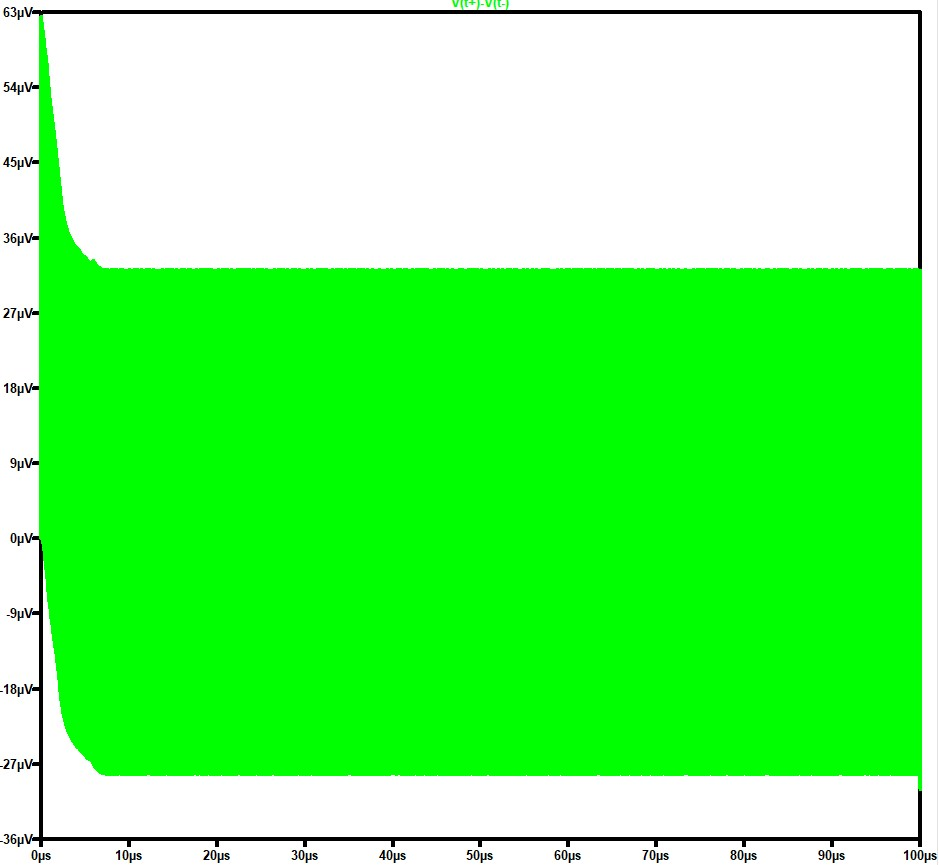
\includegraphics[width=\linewidth]{pictures/Time-Plot.jpg}
    \caption{Transient Simulation of the MAX31856 Interface}
    \label{fig:SIM}
\end{figure}

The simulated frequency response graph \cref{fig:BODE} supplies more evidence that our methods were not appropriate for creating a temperature output change. As the frequency of the induced signal increases, the response of the circuit becomes exponentially smaller. At the frequency where our experiments were operating (47MHz) the response of the MAX31856 input circuit is ~-90dB. This negative response makes creating any \ac{dc} component in the final signal very difficult.
A final mistake in our approach was the assumption that interference targeted at the thermocouple would be enough to cause output interference. There are multiple attack points just within the simple thermocouple experiments that could have been exploited. First, the MAX31856 is an IC device that has its own sensors (i.e. cold junction temperature sensor) that can be interfered with. In addition, attacks on the SPI controller as well as the microcontroller inside of device could have been explored.

\begin{figure}
    \centering
    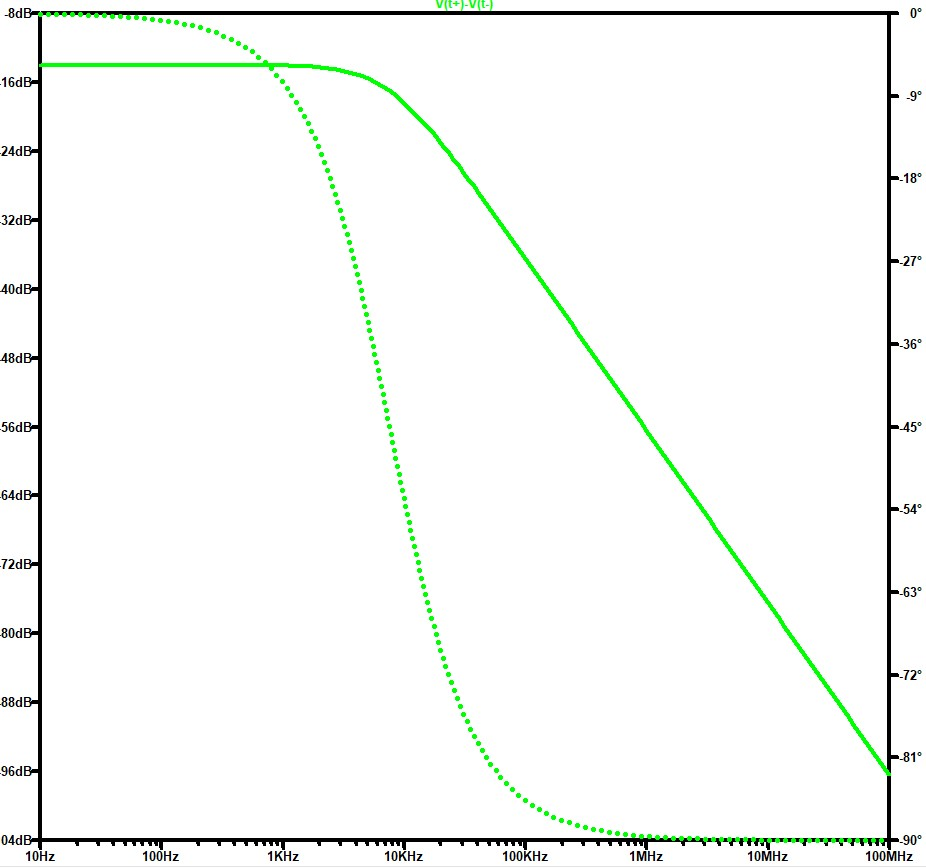
\includegraphics[width=\linewidth]{pictures/Bode.jpg}
    \caption{Bode Plot of MAX31856 Interface}
    \label{fig:BODE}
\end{figure}

\section{Software Implementation}\label{swi}
\subsection{Model Creation}\label{model-creation}
Both the simulation as well as the controller rely on a steady-state model of the thermocouple to produce realistic looking values. To do this, we used our K-Type thermocouple as a sample source for a statistical model. First, we took continuous reading over a half hour where the thermocouple and MAX31856 were at room temperature. Using Mathematica (\cref{steady-state-model-code}), we fit a distribution to the samples and created the inverse \ac{cdf} (\cref{inverse-cdf-tcouple}). Through the inverse \ac{cdf} sampling method, we could then use the resulting function as the source for our simulation. 

\begin{equation}\label{inverse-cdf-tcouple}
\begin{split}
t = x - 0.0620762 \log({-1 + 1/y}),
\end{split}
\begin{split}
t \text{- Temperature}\\
x \text{- Mean Temperature}\\
y \text{- Random number (0, 1]}
\end{split}
\end{equation}

\subsection{Controller}
To try to mitigate the effects of induced errors a rolling average was implemented in \cref{thermocouple-controller}. In addition, an upper bound and lower bound for the allowable values of the thermocouple were implemented; if the value read from the thermocouple is outside of this range, the model discussed in \cref{model-creation} is used to calculate an approximate valid value to be stored in the list of values used to calculate the rolling average.

The controller code can be run on either an Arduino or with the simulator included. This code is shown in \cref{thermocouple-controller}. All of the code written for this design and simulator, as well as a Makefile and README of how to use it can be found on github  \href{https://github.com/RSAkidinUSA/tc-volt-check}{here}\footnote{https://github.com/RSAkidinUSA/tc-volt-check}.

\subsection{Simulation}
To effectively simulate the hardware that was tested several things were needed. Firstly the simulator needed to emulate the functionality of the MAX32 thermocouple that was interfaced with by the arduino. Secondly, the simulator needed the ability to read a series of temperature values from an input file and correctly pass those along to the controller. Following proper implementation of this, functionality was added to include the ability for the simulator to modify the values that were read from the input file to simulate a thermocouple that was being attacked. This was done by forcing the values to either a lower bounded range or an upper bounded range, emulating the extreme voltages that might be induced in the device. This code is available in \cref{thermocouple-simulator}. \Cref{thermocouple-simulator-h} is the header file used to define some of the values used in the simulator.

\section{Future Work}\label{fut}
Future work would focus primarily on expanding the attack surfaces that were used for interference. As discussed in the previous section, the frequency response of the breakout circuit of the MAX31856 prevented high frequencies from being effective. In addition, alternate parts of the system need to be probed for attacks, such as the MAX31856 controller or the cold junction temperature sensor.

Exploring lower frequencies ranging from 10HZ – 10KHz would be a good staring point for future experiments. Simulation showed that this frequency range had the best response to \ac{ac} signals; although still negative \cref{fig:BODE}. Evidence that these frequencies have worked in other projects is shown in \cite{Chakraborty82,Smalcerz2013}.

Alternate emitters should also be explored. As we used a single inductor design for our emitters, we failed to explore the options that differing configurations, numbers of emitters, and inductor designs could provide. In addition, resonant and propagation interference from RF signals rather than electromagnetic inductive interference should be explored as alternate ways to create signals on the thermocouple.

Finally, many of the other components in the system could be attacks. For example, the cold junction temperature sensor on the MAX31856 board is internal which means that it expects its output to be correct for all readings. If the MAX31856 could be tricked into using values that were faulty then the temperature output would then be faulty. A similar attack could be manipulating the temperature/sensor values that are stored in internal registers. While more difficult to achieve, being able to flip register values could produce more fine-tuned interference rather than the extreme values produced by interfering with the temperature sensors.
